\chapter{Prezentarea aplicației}

In continuare voi prezenta pe scurt cele mai importante aspecte si funcționalități ale aplicației dezvolte. Pentru a putea folosi aplicația, utilizatorul trebuie să se înregistreze și să se autentifice în cadrul aplicației. După autentificare, utilizatorul va fi redirecționat către pagina principală a aplicației, unde va avea la dispozitie principalele functionalitati pentru fiecare tip de utilizator, „Walker” sau „Owner”. În continuare voi prezenta funcționalitățile oferite de aplicație pentru fiecare tip de utilizator.

\begin{figure}[!htb]
    \minipage{0.3\textwidth}
      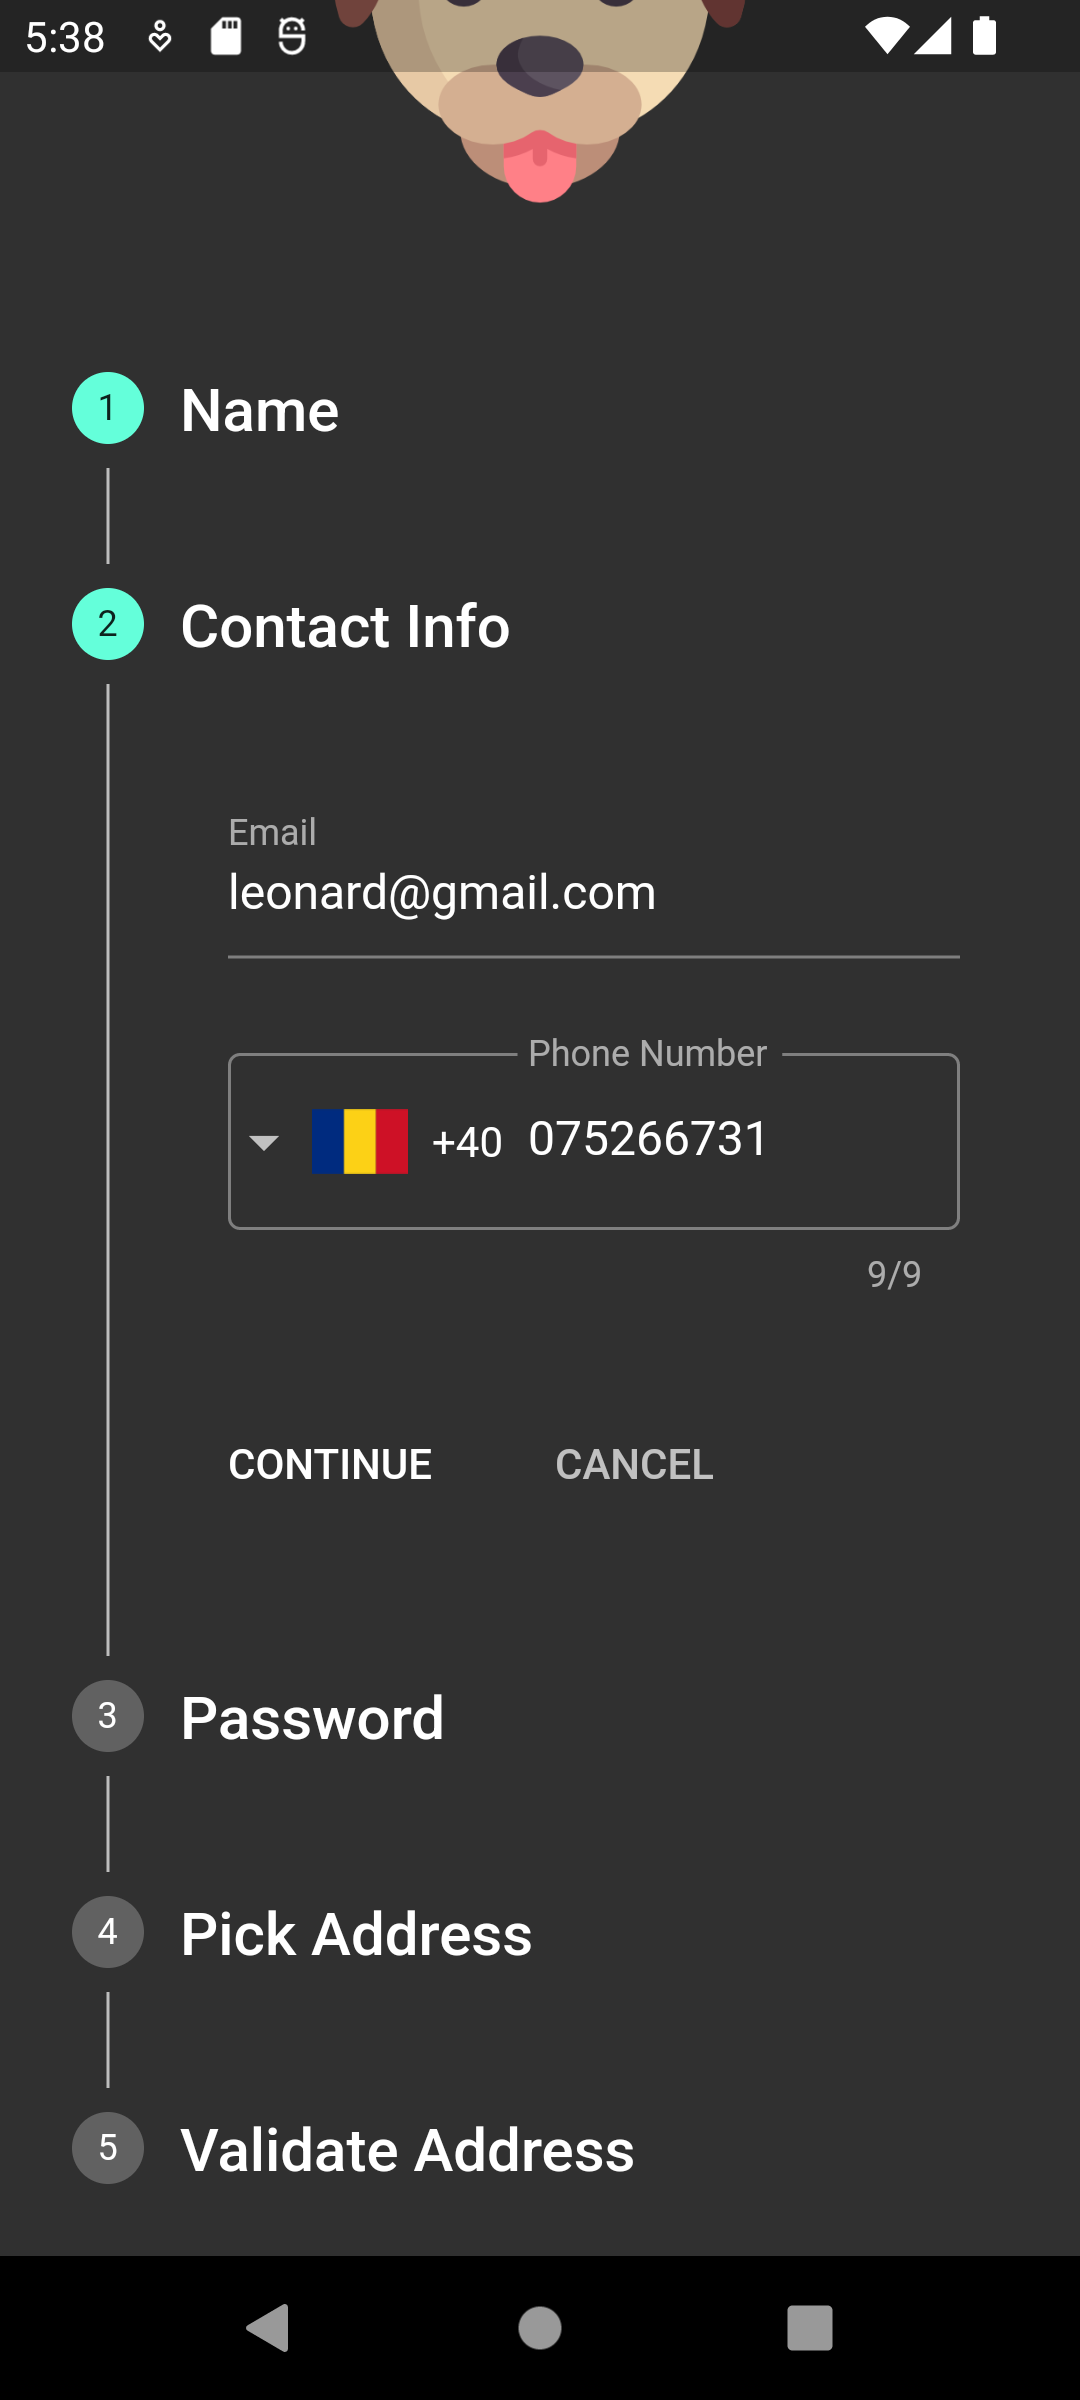
\includegraphics[width=\linewidth]{images/screenshots/register.png}
      \caption{Inregistrarea utilizatorului}\label{fig:register}
    \endminipage\hfill
    \minipage{0.3\textwidth}
      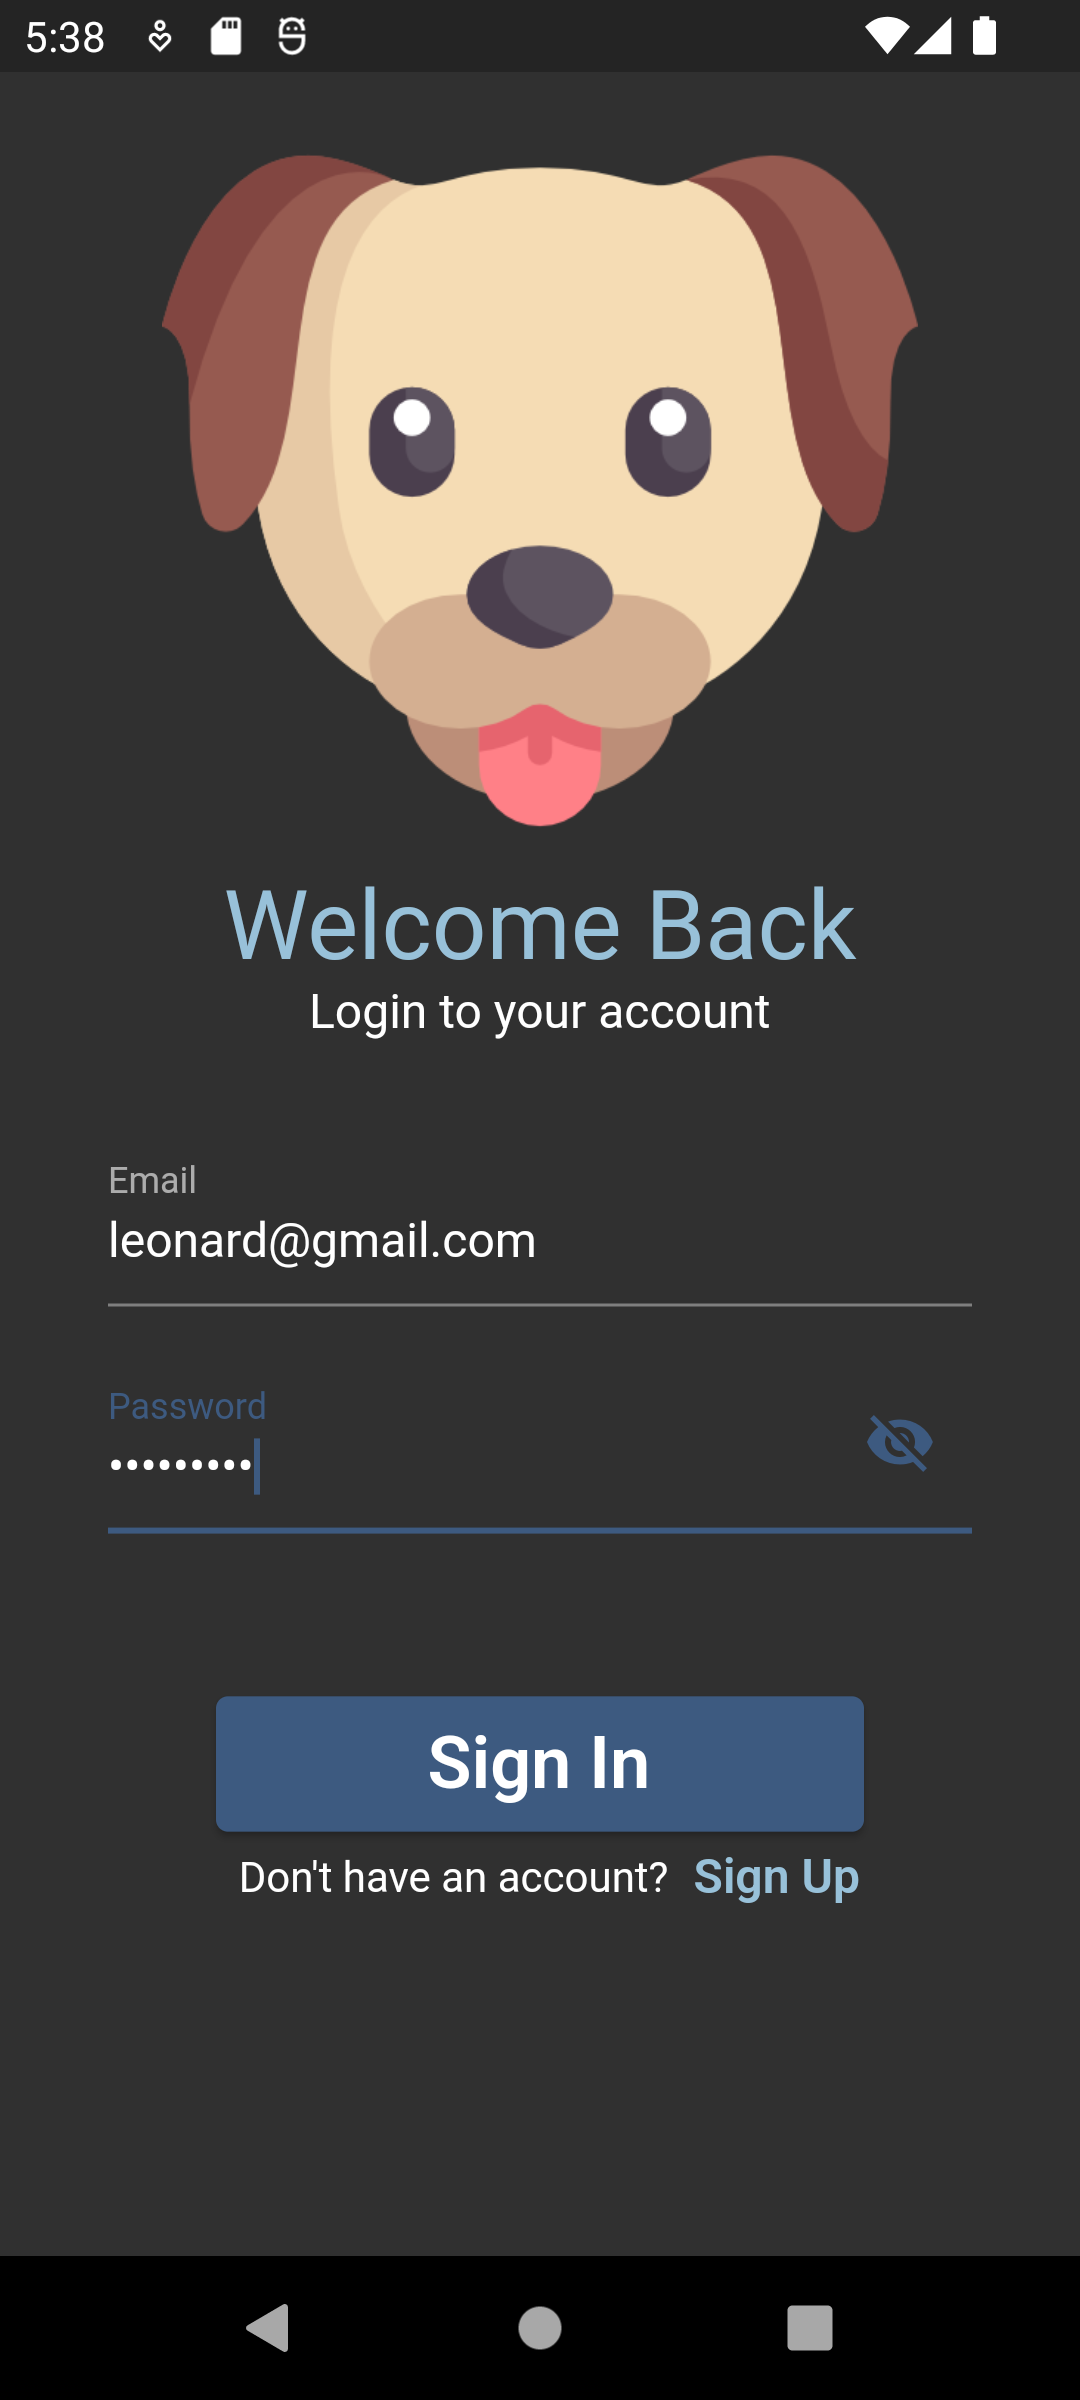
\includegraphics[width=\linewidth]{images/screenshots/login.png}
      \caption{Autentificarea utilizatorului}\label{fig:login}
    \endminipage\hfill
    \minipage{0.3\textwidth}
      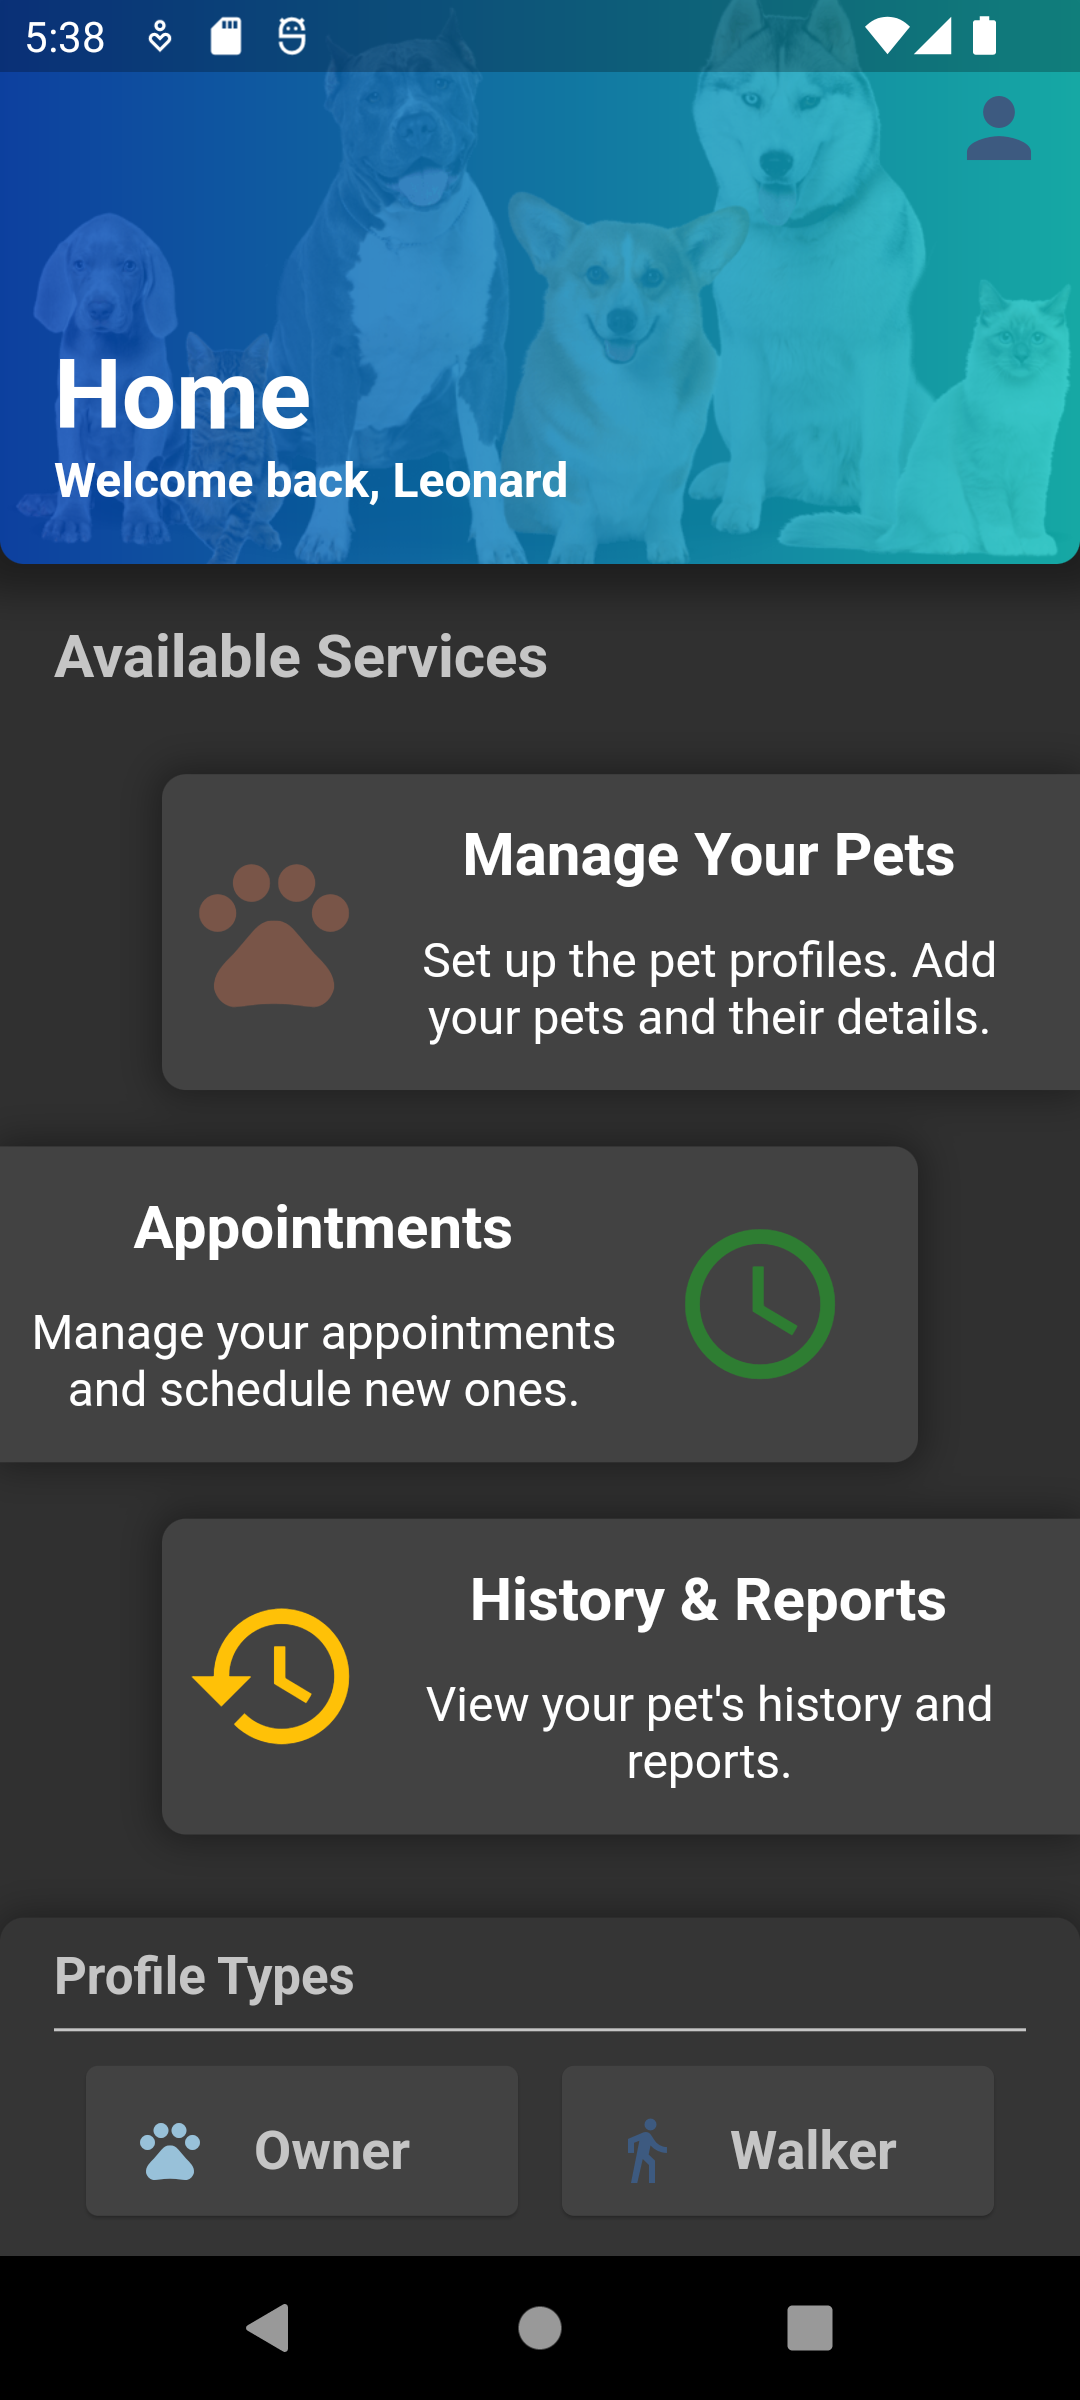
\includegraphics[width=\linewidth]{images/screenshots/main_screen.png}
      \caption{Ecranul principal}\label{fig:main_screen}
    \endminipage

\end{figure}

\section{Meniurile Owner-ului}


După ce s-a autentificat în aplicație acesta va avea la dispoziție 3 meniuri cu informații și funcționalități diferite prezente pe ecranul principal. Acestea sunt: „Manage Your Pets, „Appointments” și „History \& Reports”. În continuare voi prezența fiecare meniu în parte. 

\subsection{Manage Your Pets}

Acest meniu oferă utilizatorului posibilitatea de a vizualiza  animale de companie inregistrate de acesta în aplicație, de a adăuga un noi animale de companie, de a vizualiza informațiile despre acestea și de a edita aceste informații.

\begin{figure}[ht]
    \centering
    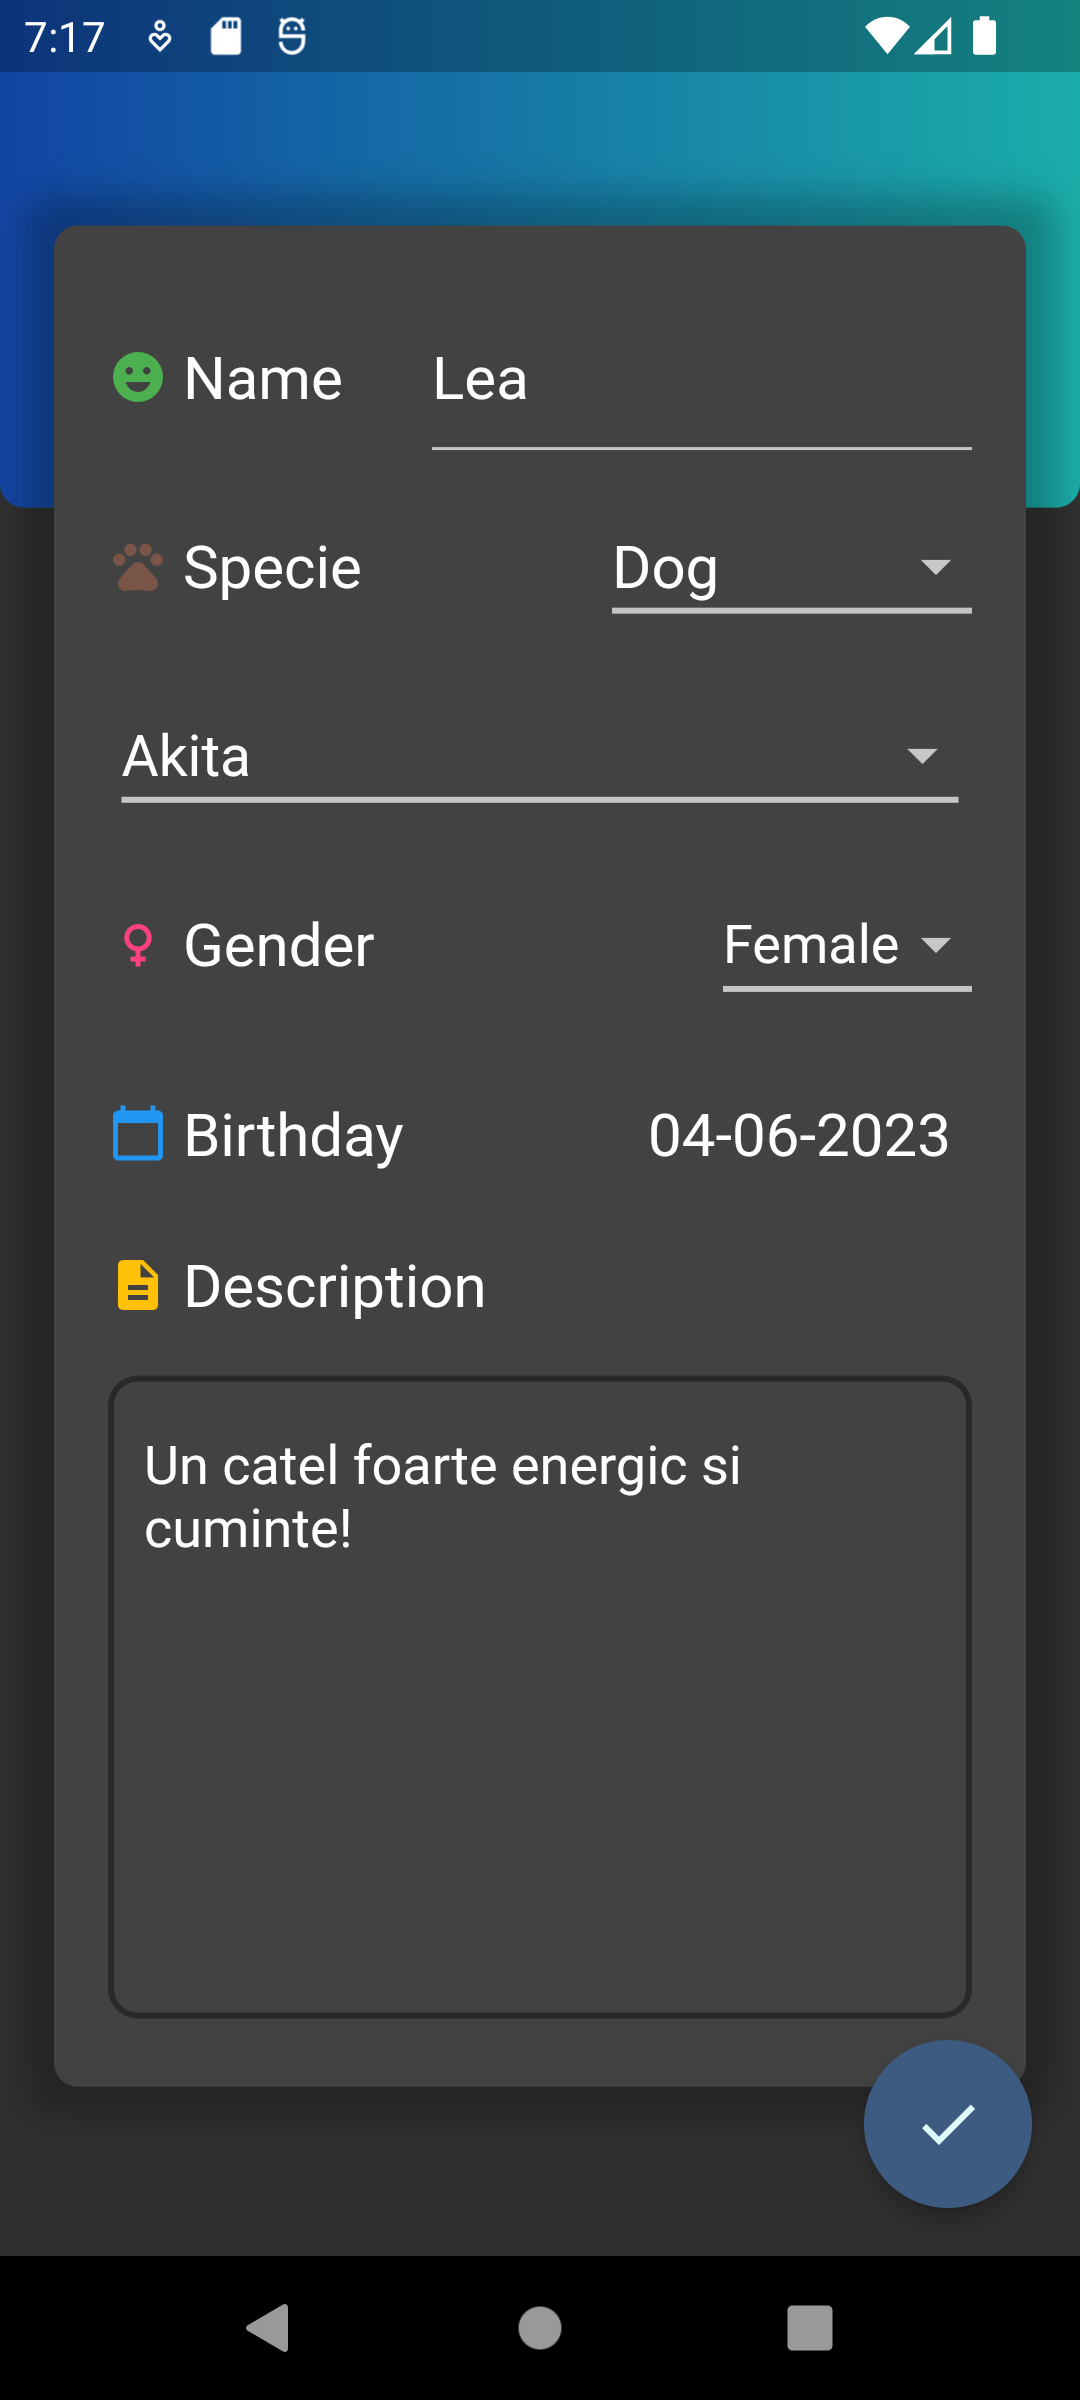
\includegraphics[width=0.4\textwidth]{images/screenshots/create_pet.png}
    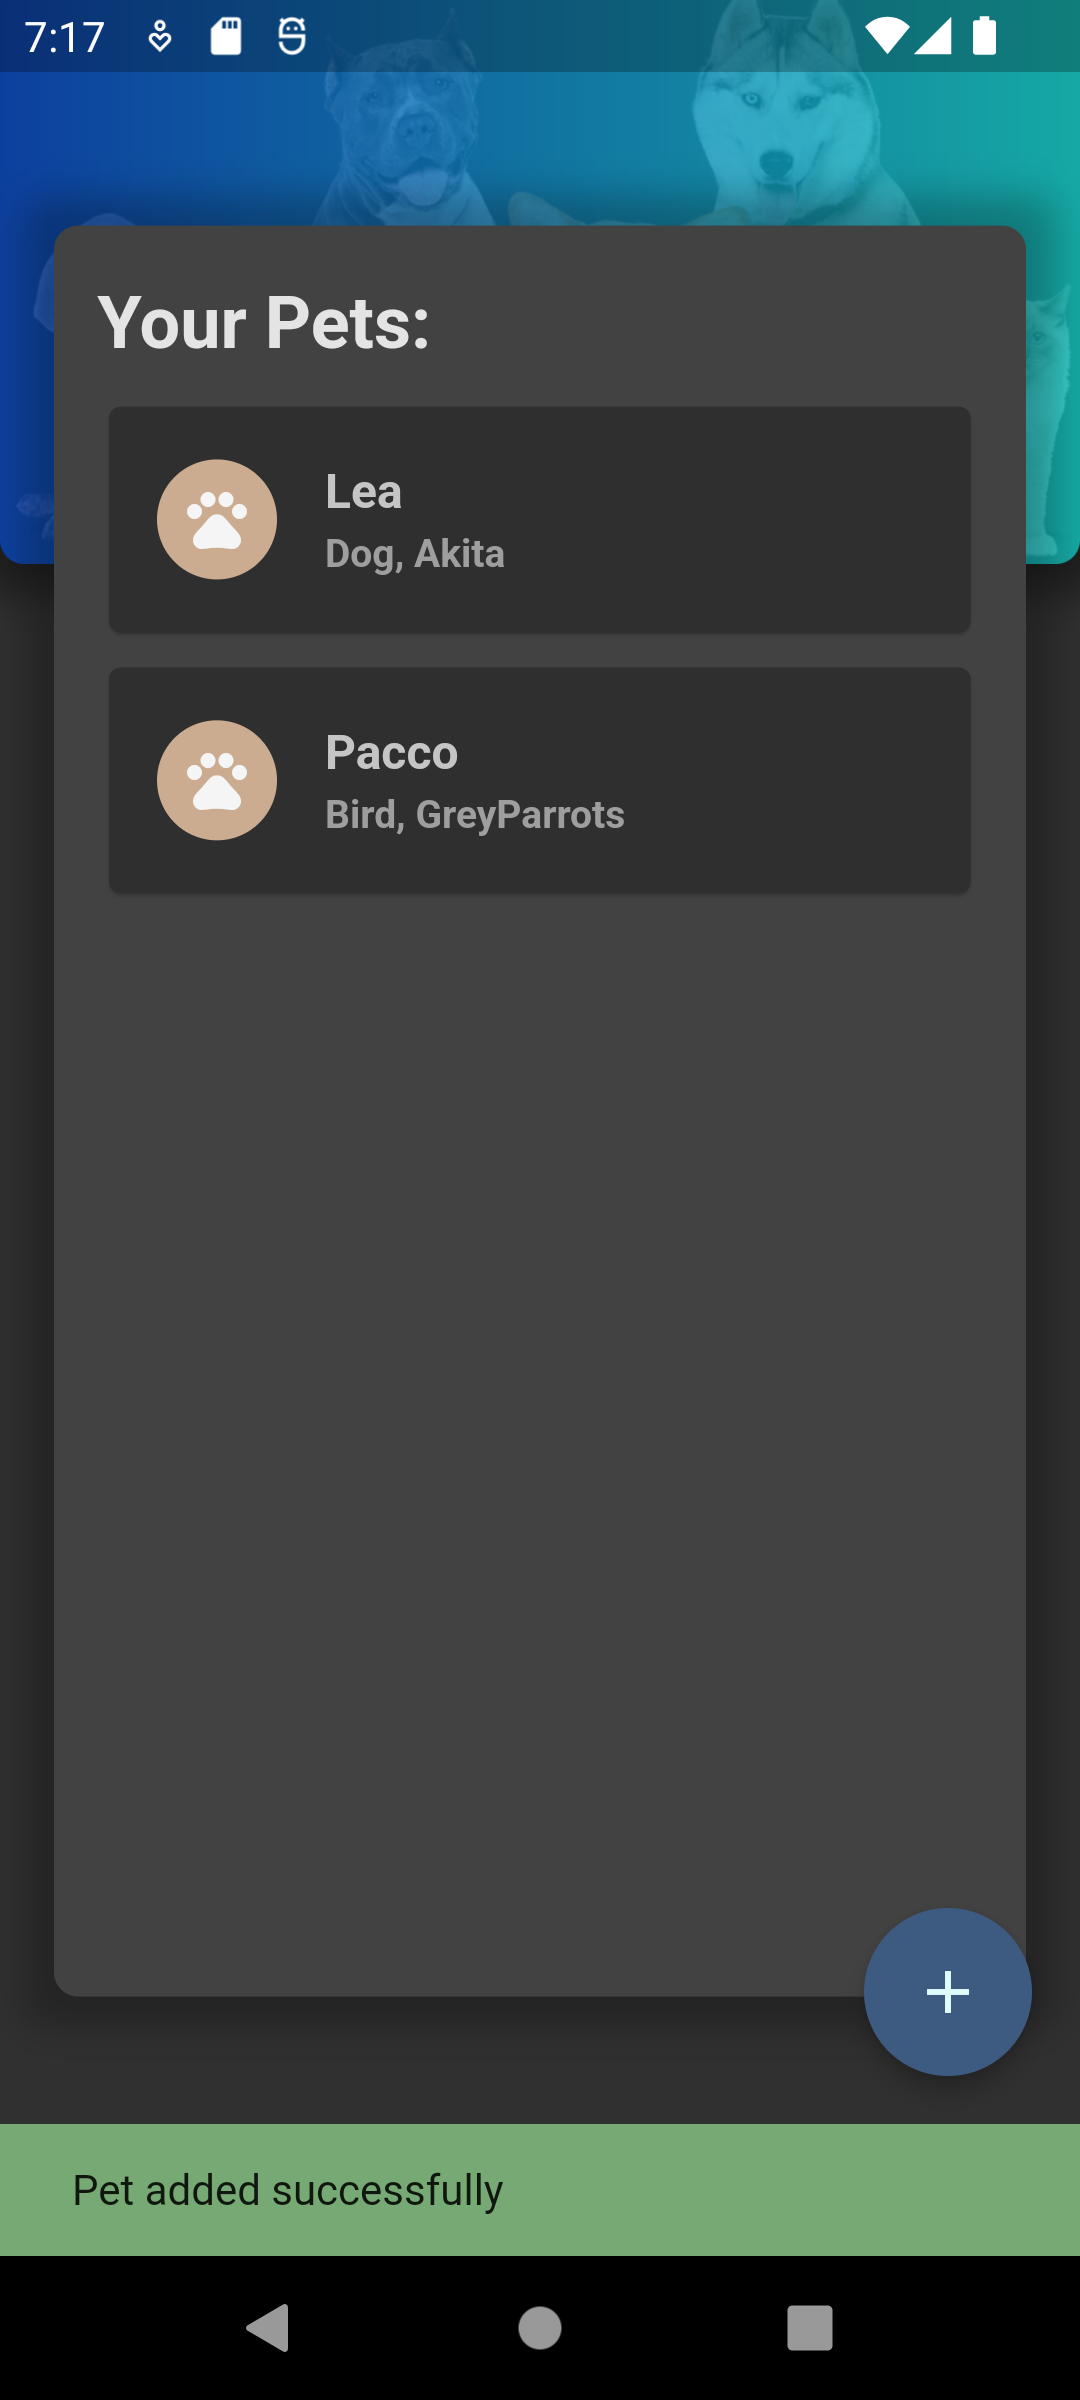
\includegraphics[width=0.4\textwidth]{images/screenshots/your_pets.png}

    \caption{Meniul „Manage Your Pets”}
    \label{fig:manage_your_pets}
\end{figure}

\subsection{Appointments}

În interiorul acesstui meniu utilizatorului are posibilitatea de a vizualiza programările curente postate de acesta și creeze noi programări. 
 
Fiecare programare care apare în acest meniu va fi insotita de un mesaj care reprezinta statusul acesteia. Statusul unei programări poate fi unul din următoarele:

\begin{itemize}
    \item \textbf{Pending} - programarea a fost postată cu succes de utilizator și se afla în așteptarea unui „Walker” care să o accepte.
    \item \textbf{Assigned} - programarea a fost acceptată de un „Walker”.
    \item \textbf{In Progress} - programarea a început și este în curs de desfășurare. Utilizatorului poate vizualiza locația curentă a „Walker-ului” pe hartă.
\end{itemize}

Tot în interiorul acestui meniul utilizatorul are posibilitatea da a posta noi anunțuri pentru una din cele 5 categori: „Walk”, „Salon”, „Sitting”, „Vet” sau „Shopping”. Fiecare categorie va fi însoțită de un button separat care va deschide un meniu în care utilizatorul va putea completă informațiile necesare pentru postarea anunțului. O dată postat anunțul, acesta va apărea în lista de programări curente și va putea fi acceptat de un „Walker”. 

\begin{figure}[ht]
    \centering
    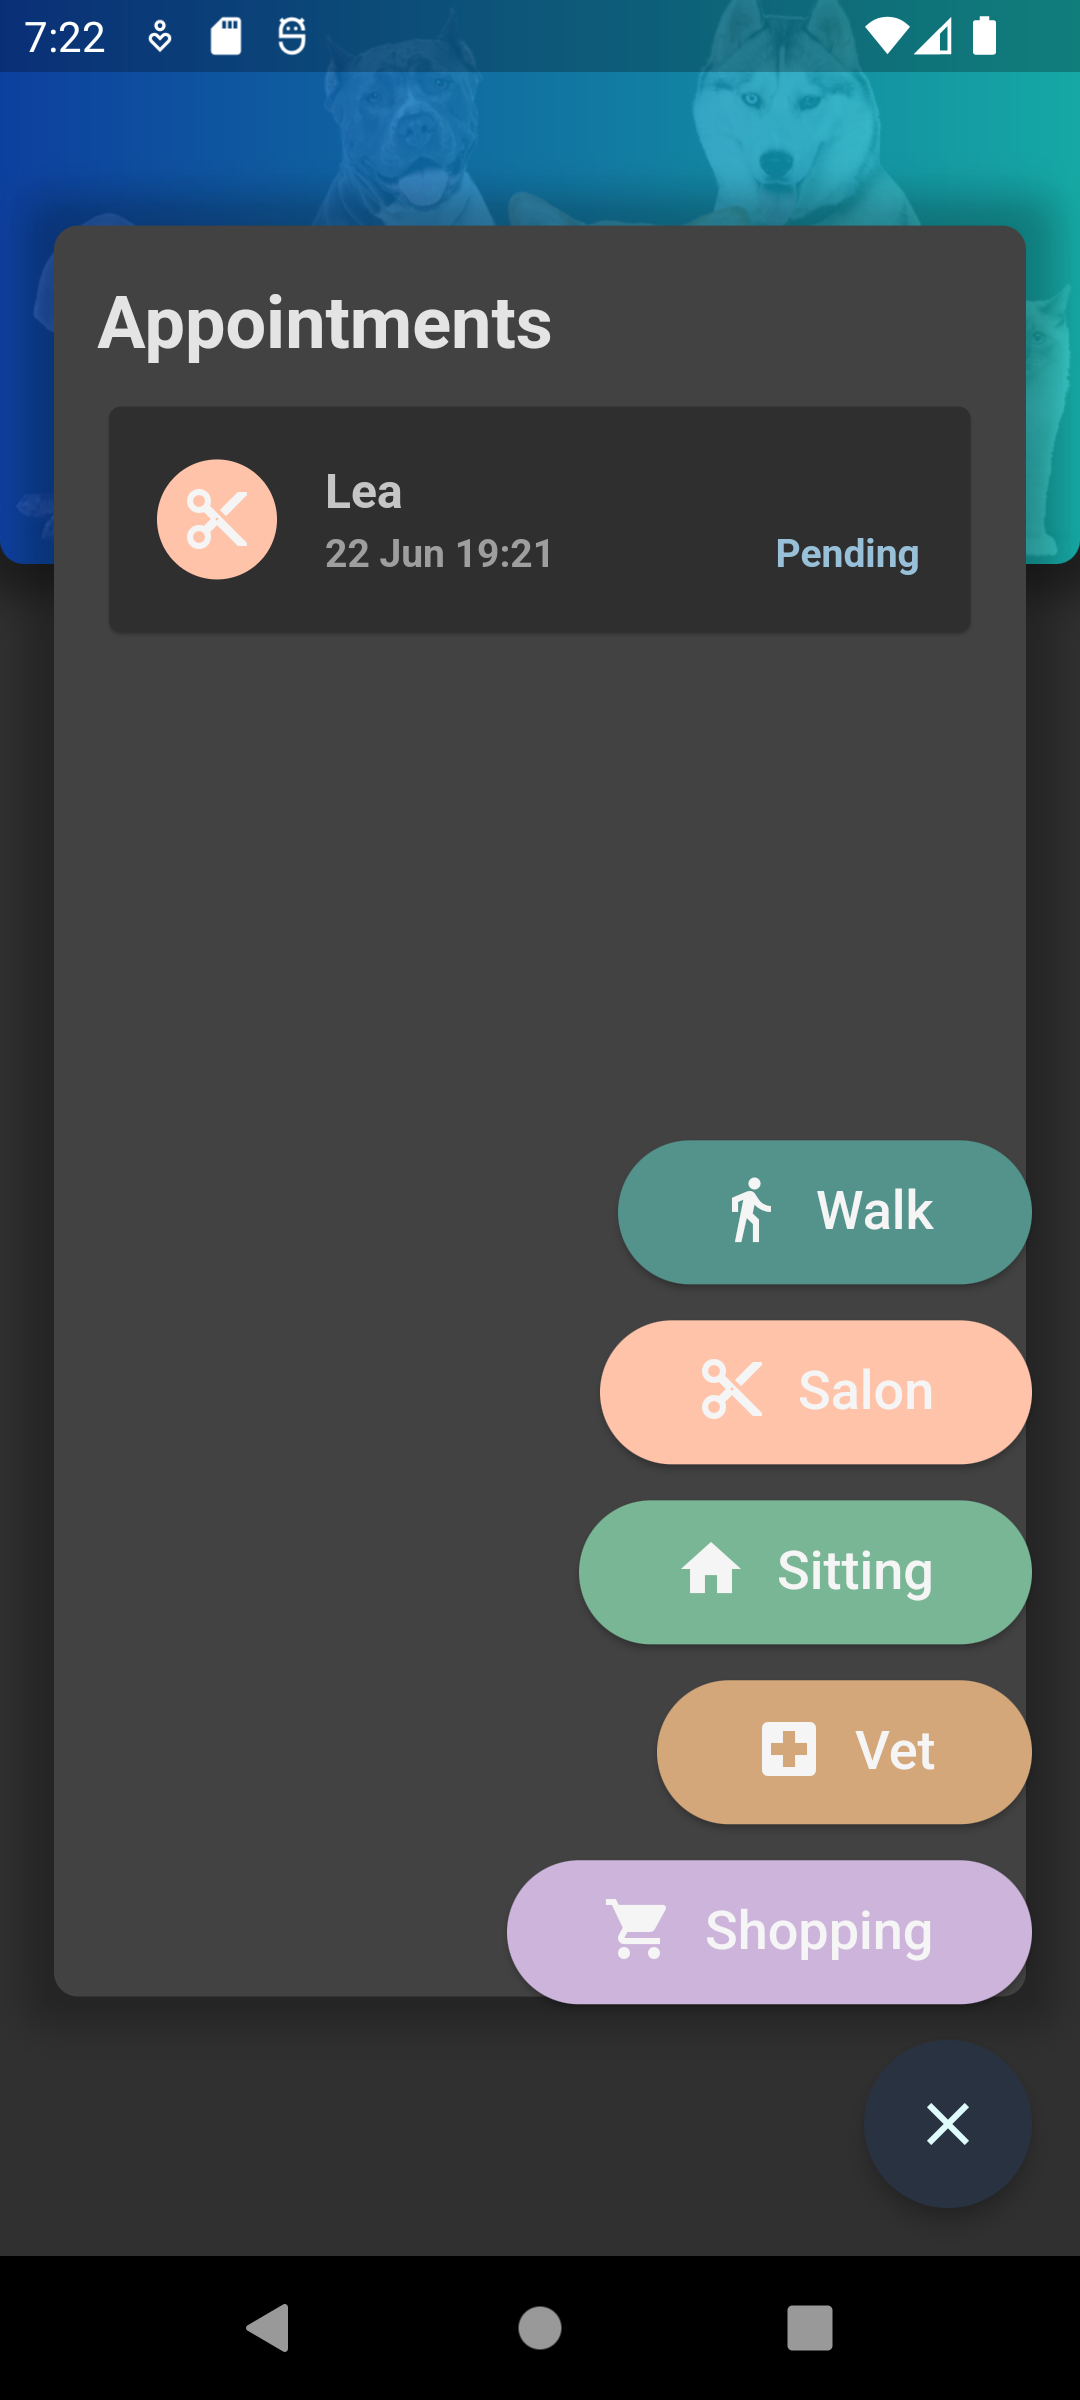
\includegraphics[width=0.23\textwidth]{images/screenshots/new_appointment.png}
    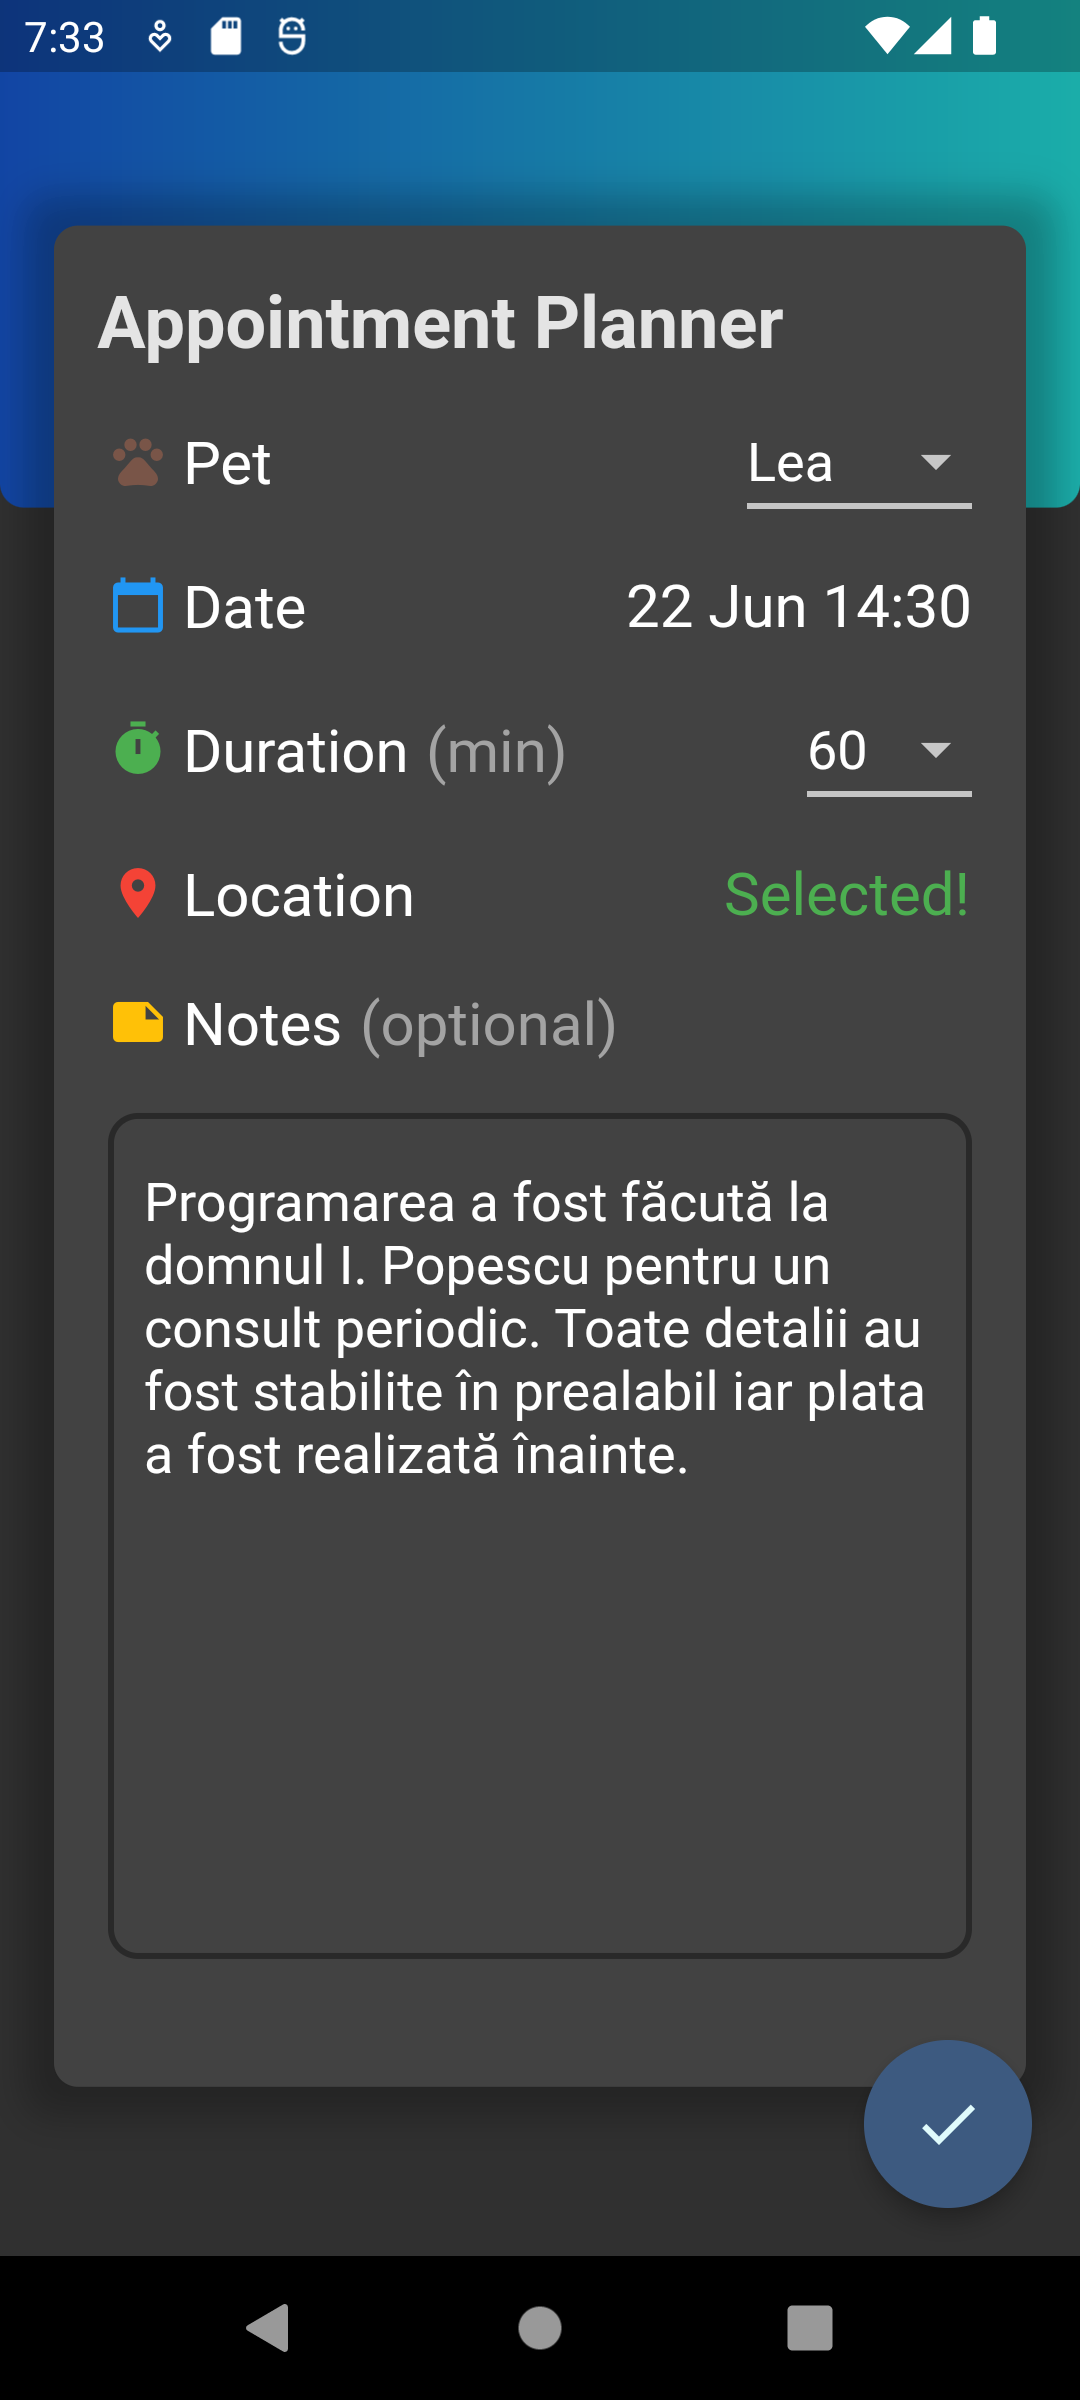
\includegraphics[width=0.23\textwidth]{images/screenshots/create_appointment.png}
    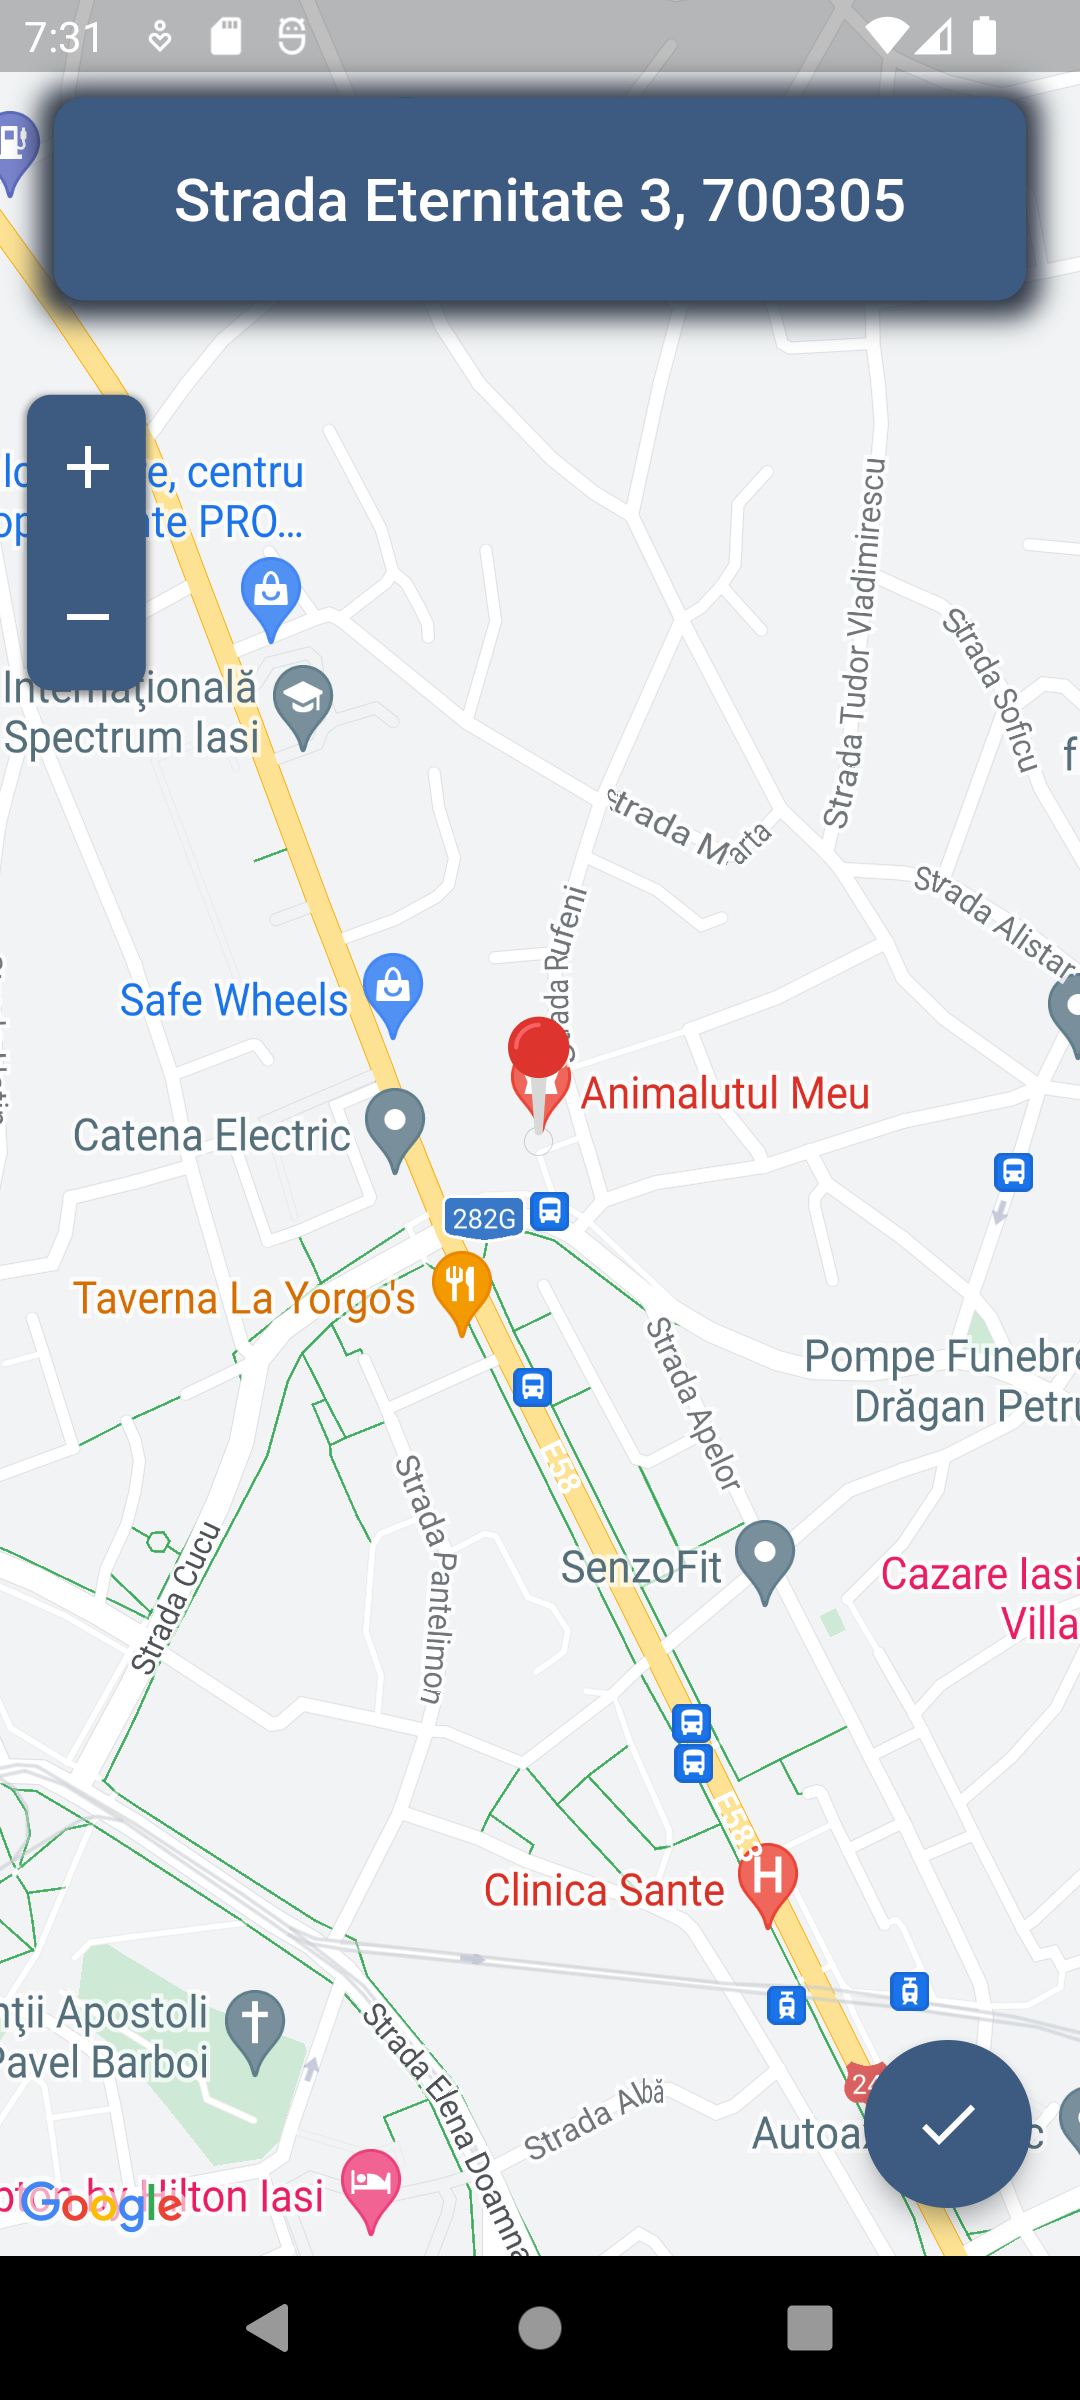
\includegraphics[width=0.23\textwidth]{images/screenshots/location_picker.png}
    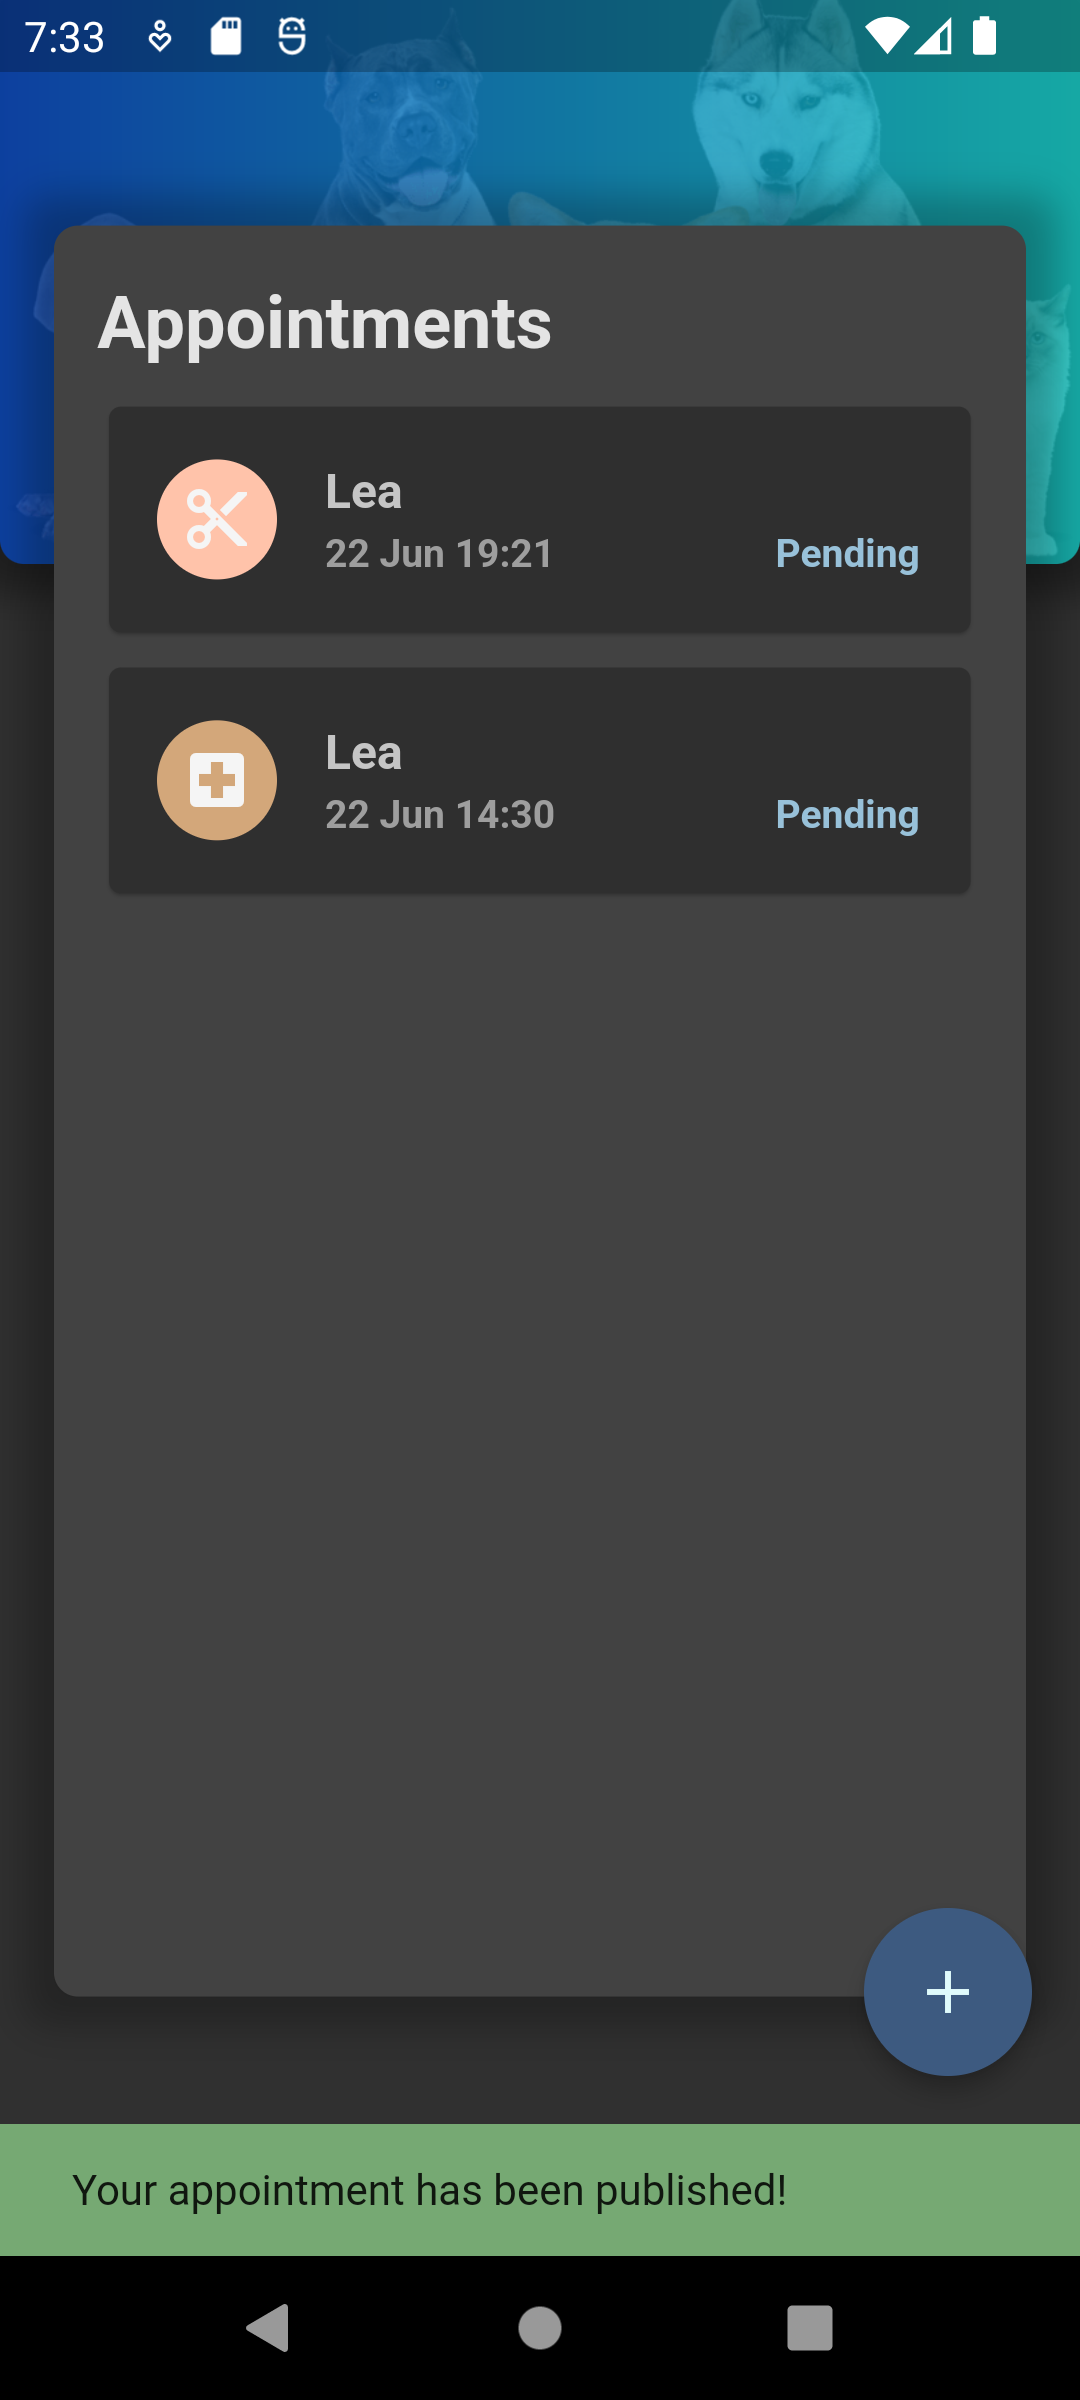
\includegraphics[width=0.23\textwidth]{images/screenshots/appointments.png}

    \caption{Meniul „Appointments”}
    \label{fig:appointments}
\end{figure}

În figura \ref{fig:appointments} se poate observă atât meniul „Appointments” care conține lista de programări curente, cât și meniul pentru crearea unei noi programări alături de pașii necesari pentru crearea acesteia. Tot aici se poate observă utilizarea a trei dintre servicii externe amintite anterior, Google Maps, Geolocator și Geocoding. Primul folosit pentru a afișarea hărții, al doilea pentru a determina locația curentă a utilizatorului și al cel din urmă pentru a determina adresa și informațiile locației selectate de utilizator pe harta.

\subsection{History \& Reports}

Acest meniu oferă utilizatorului posibilitatea de a vizualiza istoricul programărilor postate de acesta și indeplinite de un „Walker”. 

\section{Meniurile Walker-ului}

\begin{wrapfigure}[9]{r}{0.4\textwidth}
    \centering
    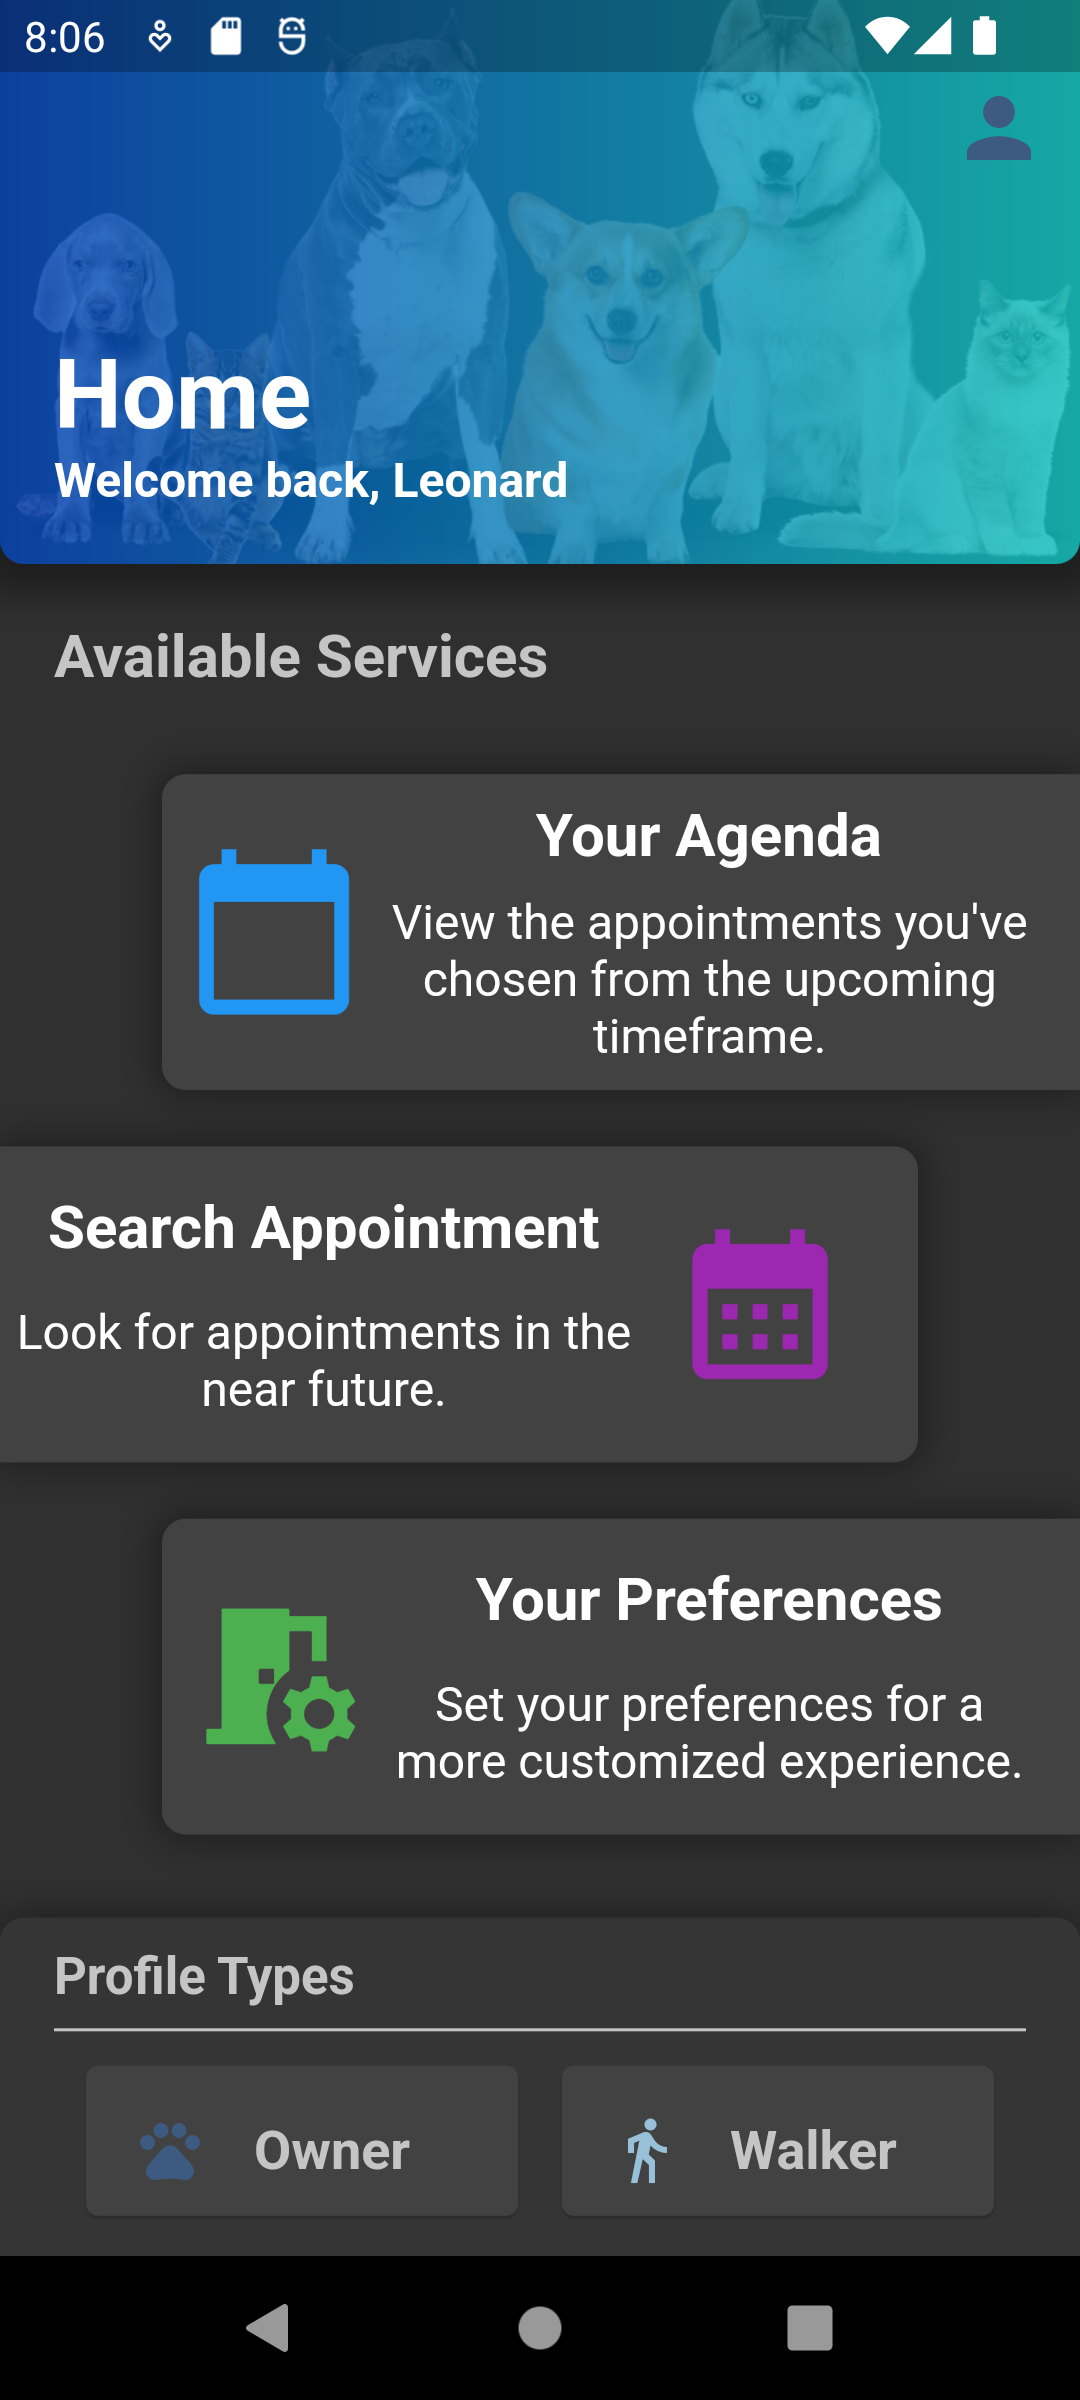
\includegraphics[width=0.4\textwidth]{images/screenshots/main_menu_walker.png}
    \caption{Meniul principal al „Walker-ului”}
    \label{fig:main_menu_walker}
\end{wrapfigure}

Utilizatorul poate acesa meniu-urile „Walker-ului” și meniurile sale prin intermediul butoanelor din meniul „Profile Types” din partea inferioară a ecranului principal. O dată ce a fost selectat unul din profile, utilizatorul va fi redirecționat către ecranul principal al profilului selectat. Aici se afla 3 meniuri diferite, meniul „Your Agenda”, „Search Appointment” și „Your Preferences”. În continuare voi prezenta fiecare meniu în parte.

\newpage

\subsection{Search Appointment}

În acest meniu vor apărea programările postate de utilizatorii și pe care „Walker-ul” le poate acceptă. Acestea sunt sortate după preferințe și apar în ordinea în care acestea ar trebui îndeplinite. De aici „Walker-ul” le poate sorta manual și să își aleagă programările care îi sunt pe plac și i-ar face plăcere să le îndeplinească. 

   
Tot aici se află și butonul pentru generarea unei liste de programări personalizate. Acesta va deschide un meniu în care utilizatorul va trebui să specifice modul în care se va deplasa între programări, cu mașina sau pe jos, și ziua pentru care se dorește generarea. După ce a fost generată lista, aceasta va trebui să fie acceptată de utilizator pentru ca ele sa fie adăugate în lista sa de programări. Toate programările acceptate de utilizator vor fi vizibile în meniul „Your Agenda”.

\begin{figure}[ht]
    \centering
    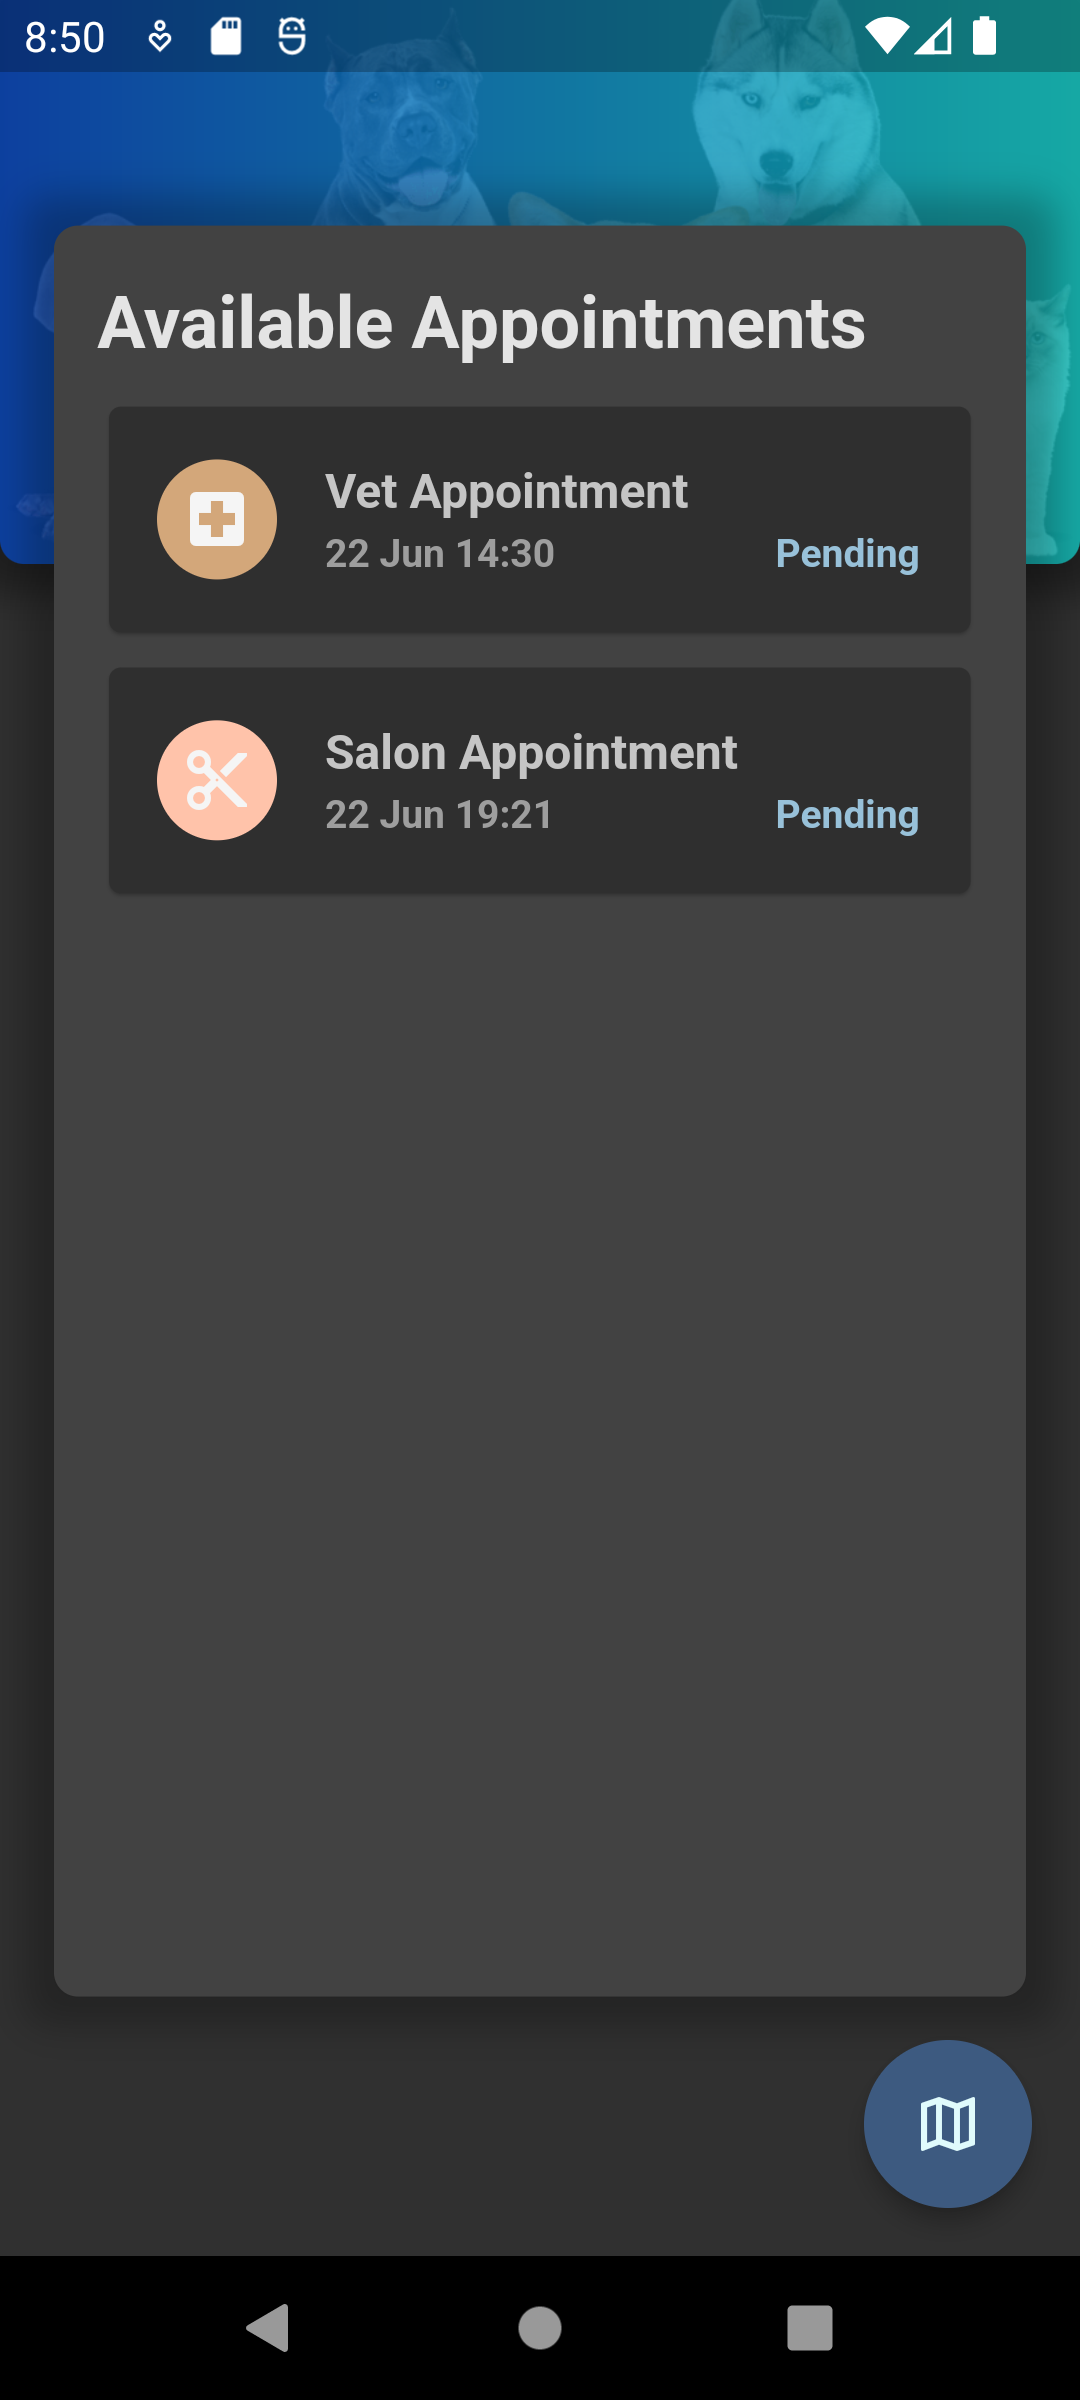
\includegraphics[width=0.23\textwidth]{images/screenshots/available_appointments.png}
    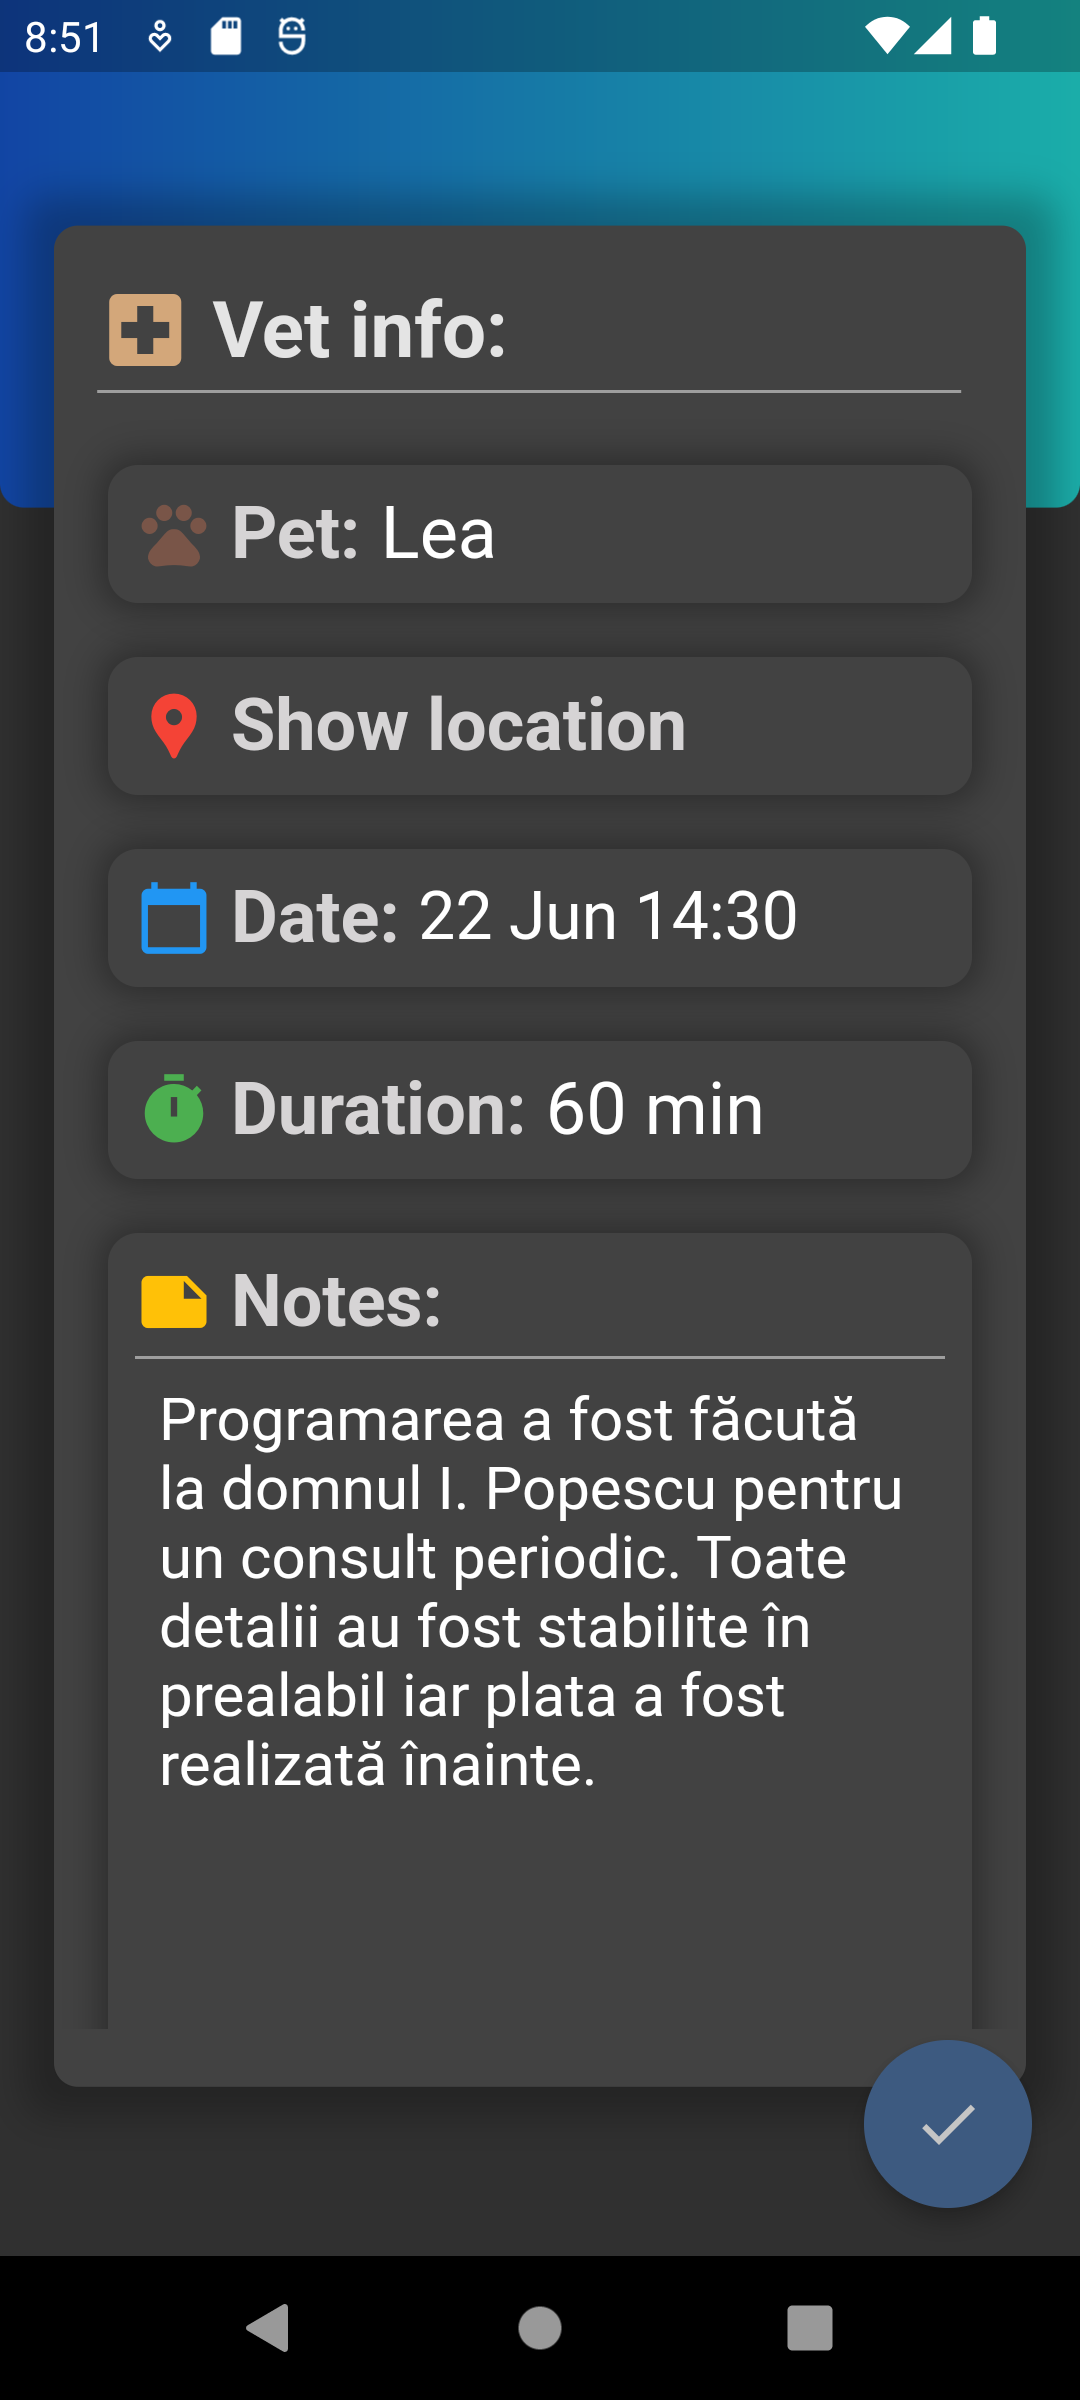
\includegraphics[width=0.23\textwidth]{images/screenshots/appointment_info.png}
    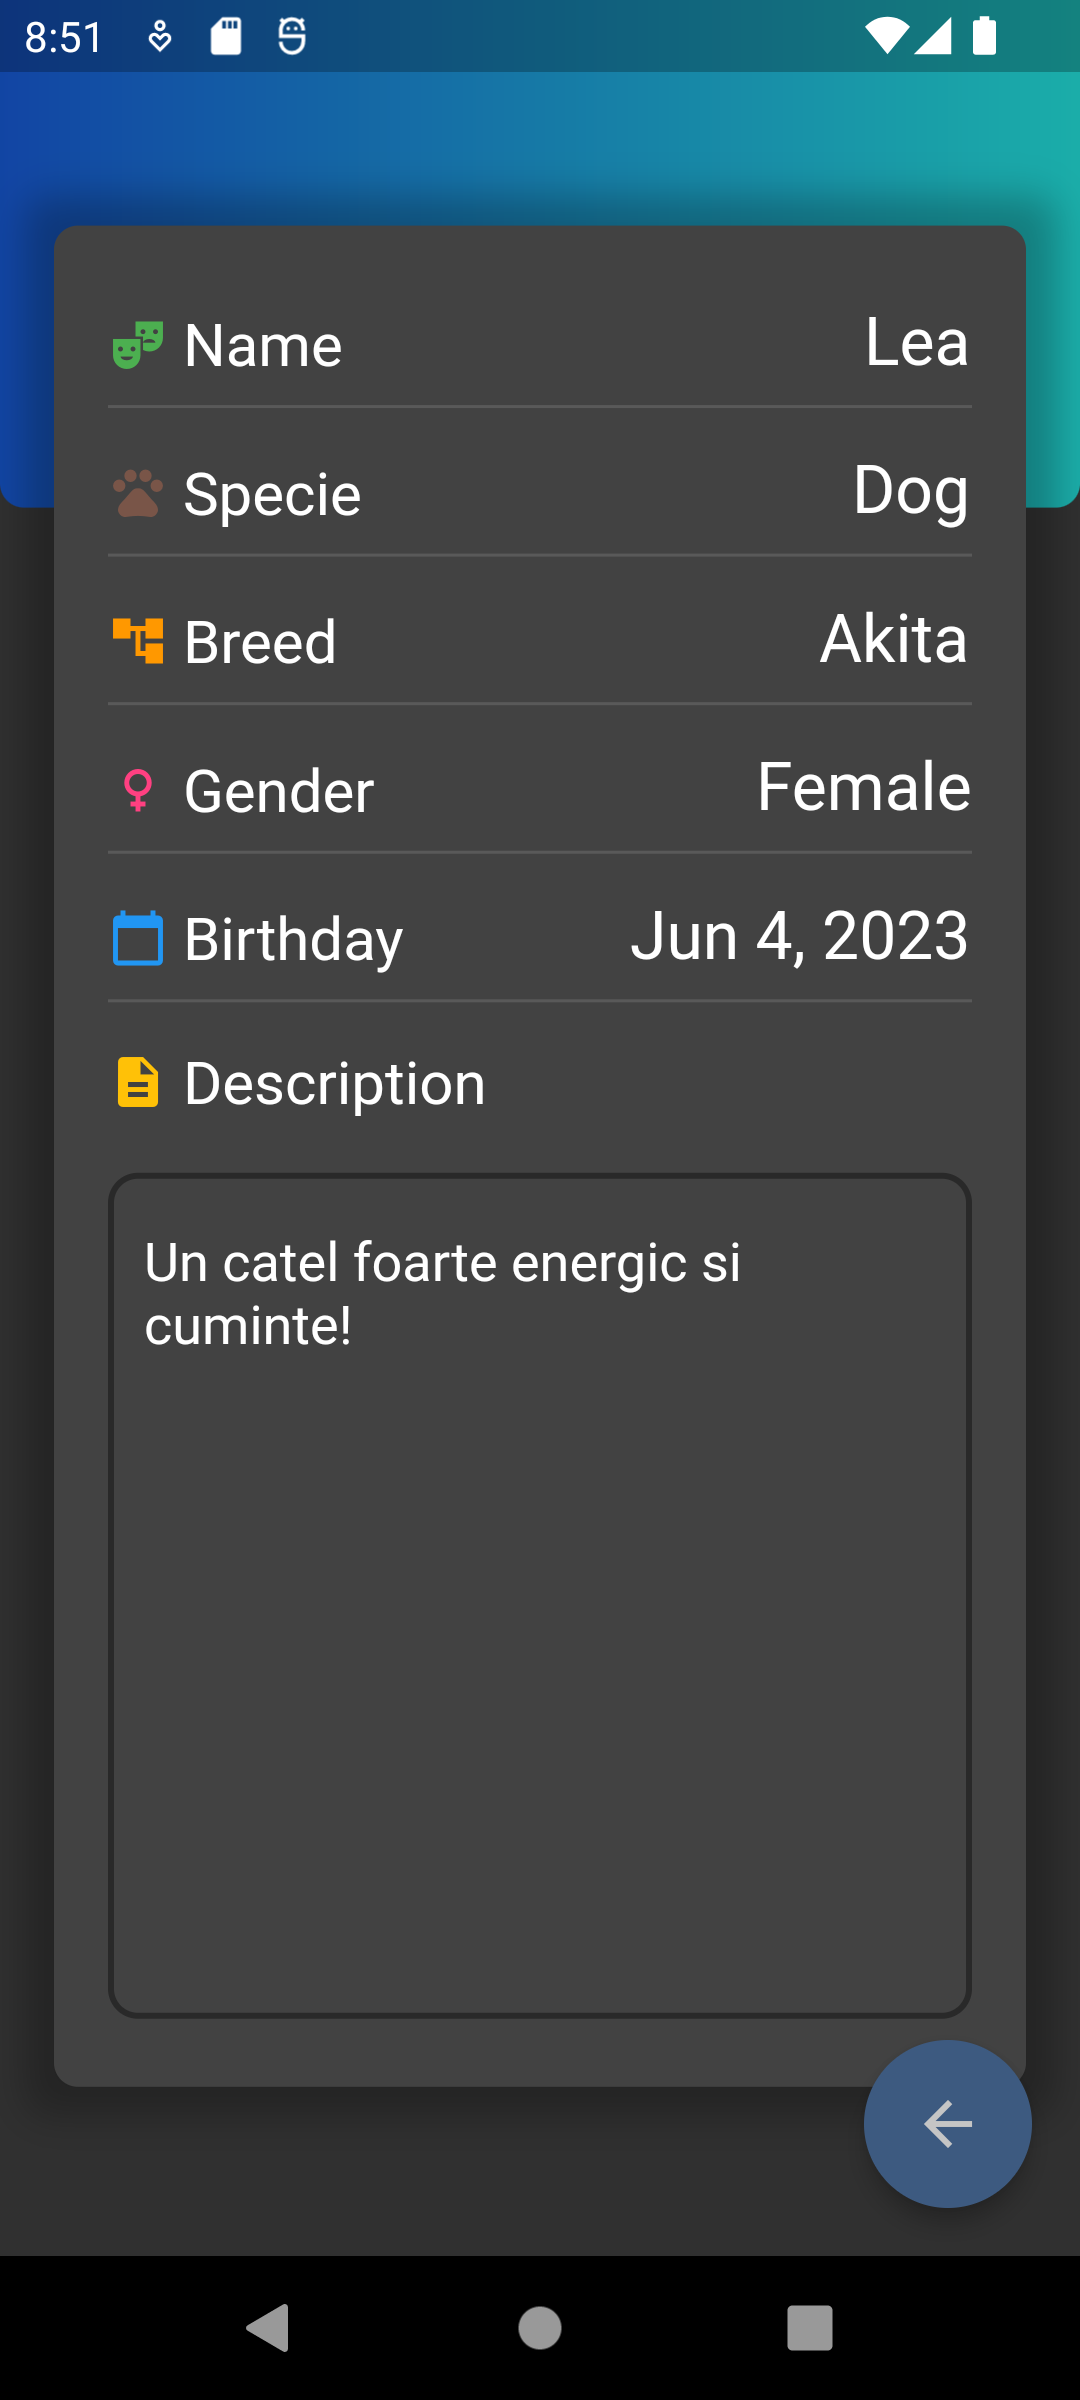
\includegraphics[width=0.23\textwidth]{images/screenshots/pet_info.png}
    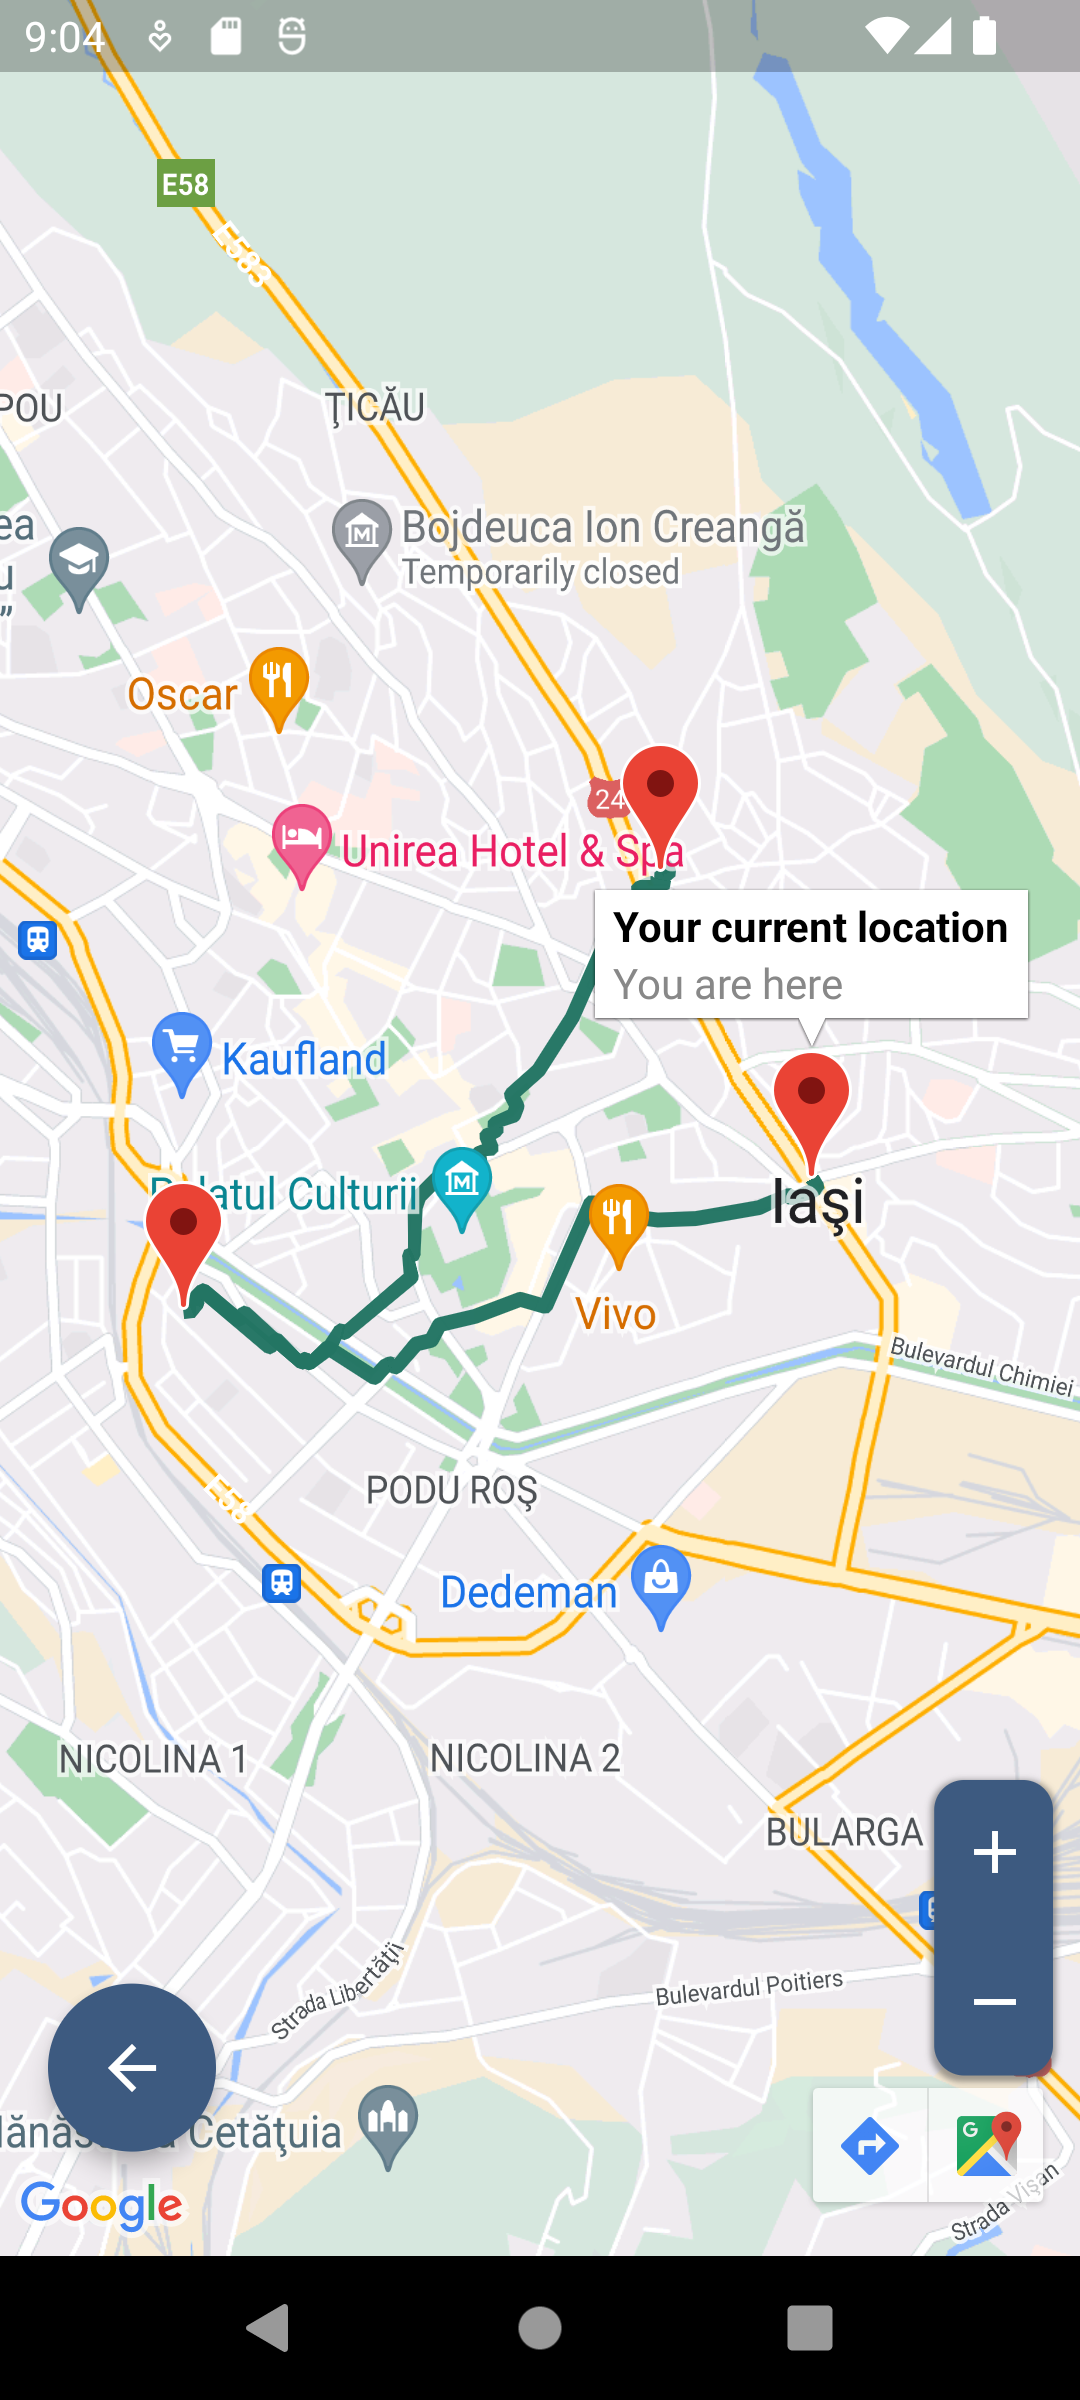
\includegraphics[width=0.23\textwidth]{images/screenshots/show_location.png}
    \caption{Meniul „Search Appointment”}
    \label{fig:schedule_appointment}
\end{figure}

În figura \ref{fig:schedule_appointment} se poate observă meniul „Search Appointment” care conține lista de programări disponibile. Dând click pe o programare va apărea un meniu pentru vizualizarea informațiilor despre programarea selectată. Din acest meniu putem vizualiza informațiile despre animalul de companie pentru care se face programarea, dată și durata programări, unde data reprezintă momentul în care animalul trebuie să fie prezent la medic iar durata reprezintă timpul necesar consultației. Tot aici putem vizualiza și o harta care include locația unde se află animalul de companie și de unde trebuie ridicat alături de locația unde acesta trebuie să ajungă. Pentru a ușura muncă „Walker-ului” am generat și drumul minim pe care acesta trebuie să îl parcurgă de la locația sa actuala până la cele două locații menționate anterior. Drumul generat în poză a patra a fost generat pentru a fi parcurs pe jos. Pentru fiecare punct de pe harta a fost calcula și distanță alături timpul necesar pentru a ajunge la el de la punctul anterior.

\subsection{Your Preferences}

\begin{wrapfigure}[13]{r}{0.4\textwidth}
    \centering
    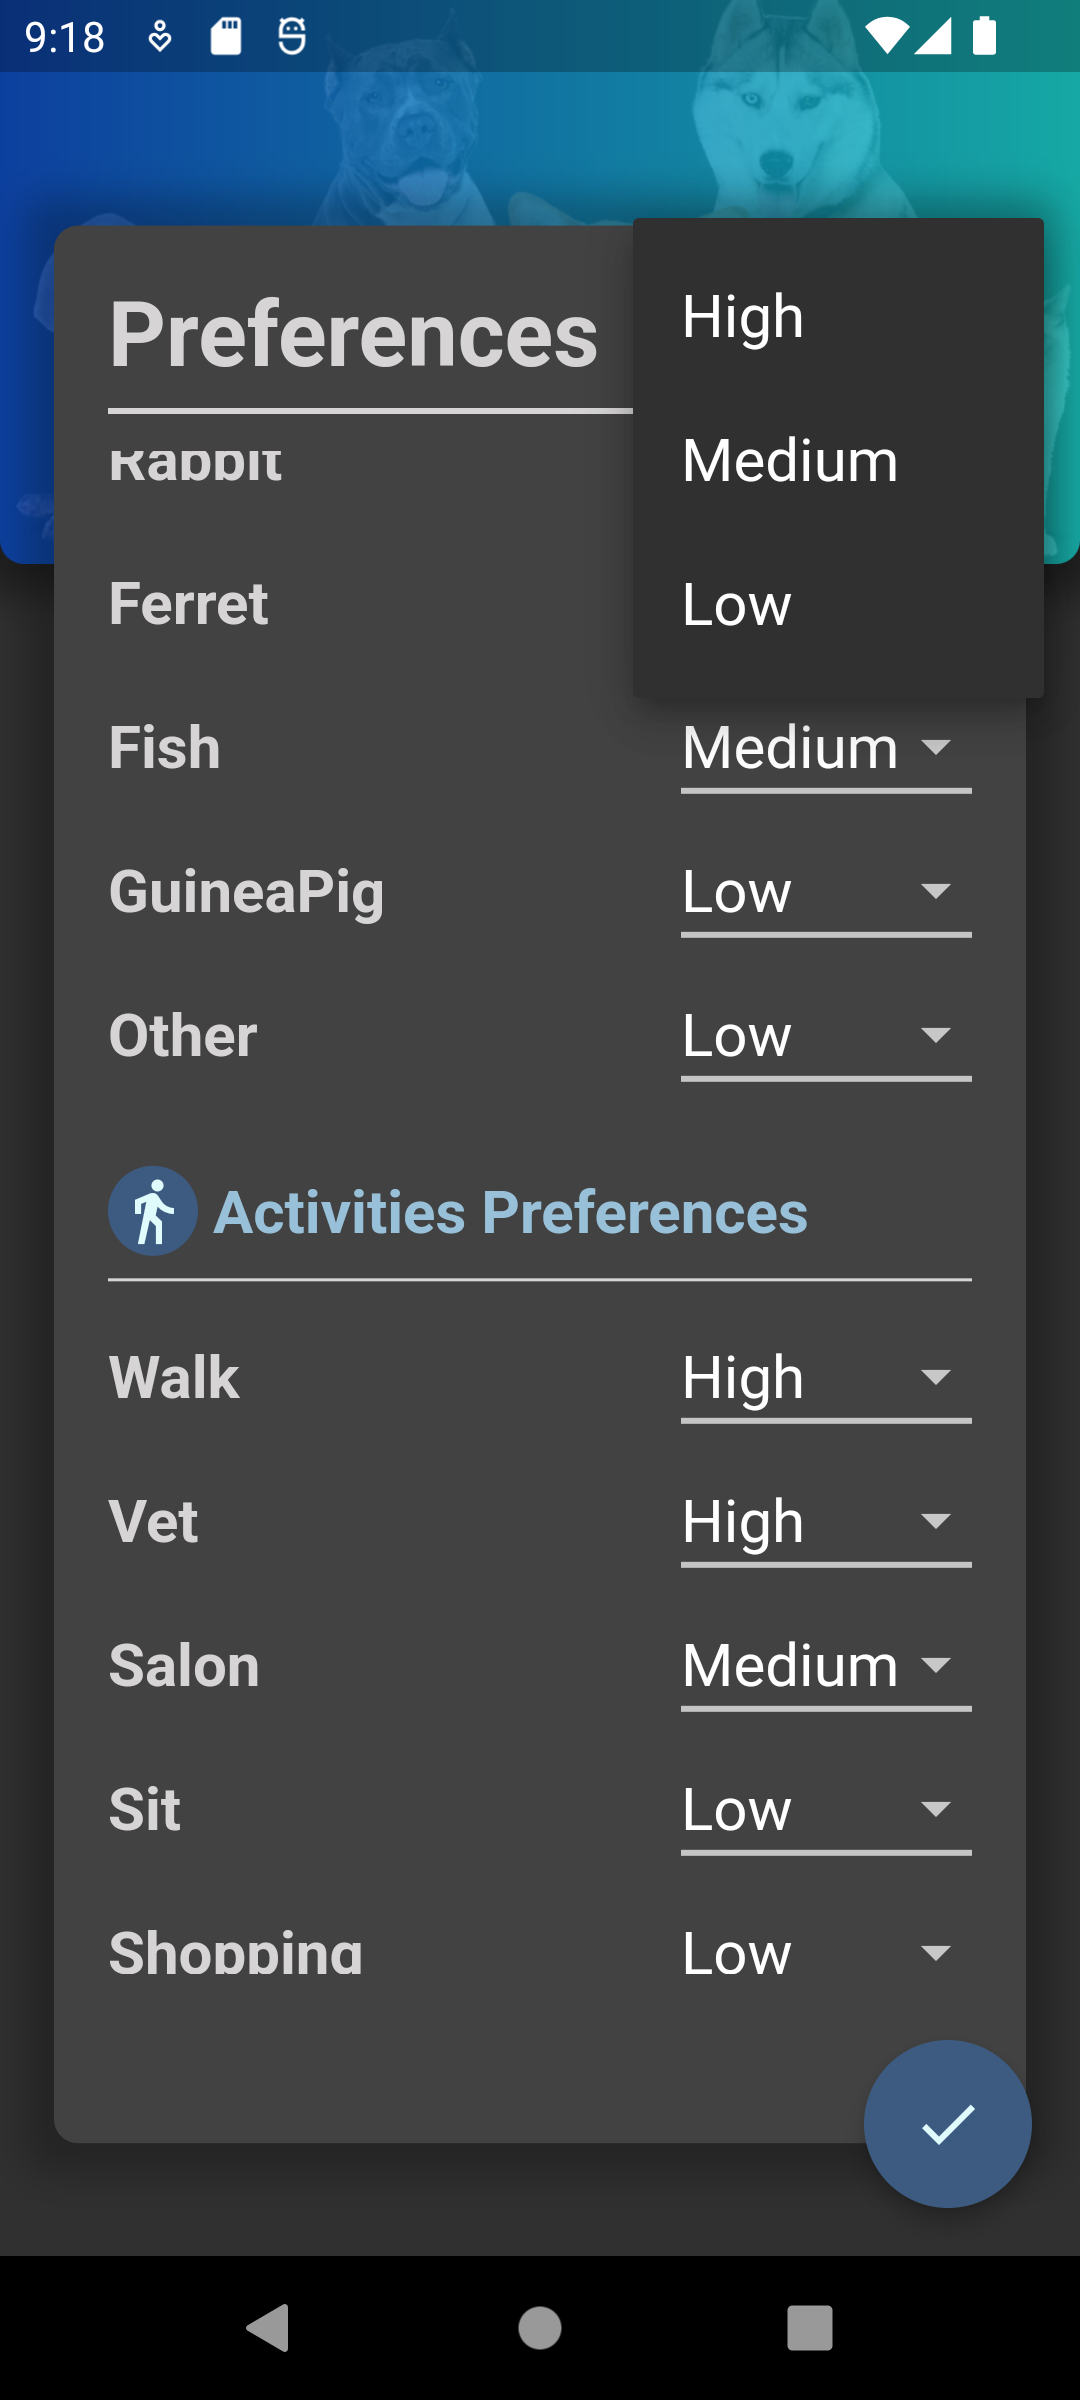
\includegraphics[width=0.4\textwidth]{images/screenshots/preferences.png}
    \caption{Meniul \newline „Your Preferences”}
    \label{fig:your_preferences}
\end{wrapfigure}

Acest meniu oferă utilizatorului posibilitatea de a vizualiza preferințele și de a le edita. Preferințele sunt împărțite în 2 categorii: preferințe pentru animalele de companie și preferințe pentru programări. Pentru fiecare element din aceste categorii utilizatorul poate alege unul din cele 3 niveluri de preferințe:

\begin{itemize}
    \item \textbf{Low} - utilizatorul nu ar prefera sa aibă de a face cu acest element.
    \item \textbf{Medium} - utilizatorul este indiferent în ceea ce privește acest element.
    \item \textbf{High} - utilizatorul ar dori să aibă de a face cu acest element.
\end{itemize}

\newpage

\subsection{Your Agenda}

Acest meniu oferă utilizatorului posibilitatea de a vizualiza agenda sa. Aici se află programările acceptate de acesta și care se află în curs de așteptare. De aici utilizatorul poate începe o programare dând click pe această iar în acel moment harta va fi încărcată iar locația sa va fi urmărită constant. De acum sarcina „Walker-ul” este de a ajunge la locația indicată pe hartă unde se află animalul de companie și după în după în funcție de fiecare tip de programare va avea o sărină diferită de inplinit. 


\begin{itemize}
    \item \textbf{Walk} - „Walker-ul” trebuie să plimbe animalul de companie pentru perioada de timp specificată în programare și să îl aducă înapoi la locația de unde l-a preluat după ce a expirat timpul.
    \item \textbf{Salon | Vet} - „Walker-ul” trebuie să ducă animalul de companie la locația indicată pe hartă și să îl aștepte până când programarea este finalizată. După ce programarea este finalizată, „Walker-ul” trebuie să îl aducă înapoi la locația de unde l-a preluat. 
    \item \textbf{Sitting} - „Walker-ul” trebuie să aducă animalul de companie la el acasă și să aibe grijă de acesta până când programarea este finalizată. După ce programarea este finalizată, „Walker-ul” trebuie să îl aducă înapoi la locația de unde l-a preluat.
    \item \textbf{Shopping} - „Walker-ul” trebuie să meargă la locația indicată pe hartă și să predee produsele comandate de utilizator. Produse trebuie cumpărate de „Walker” inainte iar costul acestora va fi rambursat de către utilizator.
\end{itemize}

\newpage

\begin{figure}[ht]
    \centering
    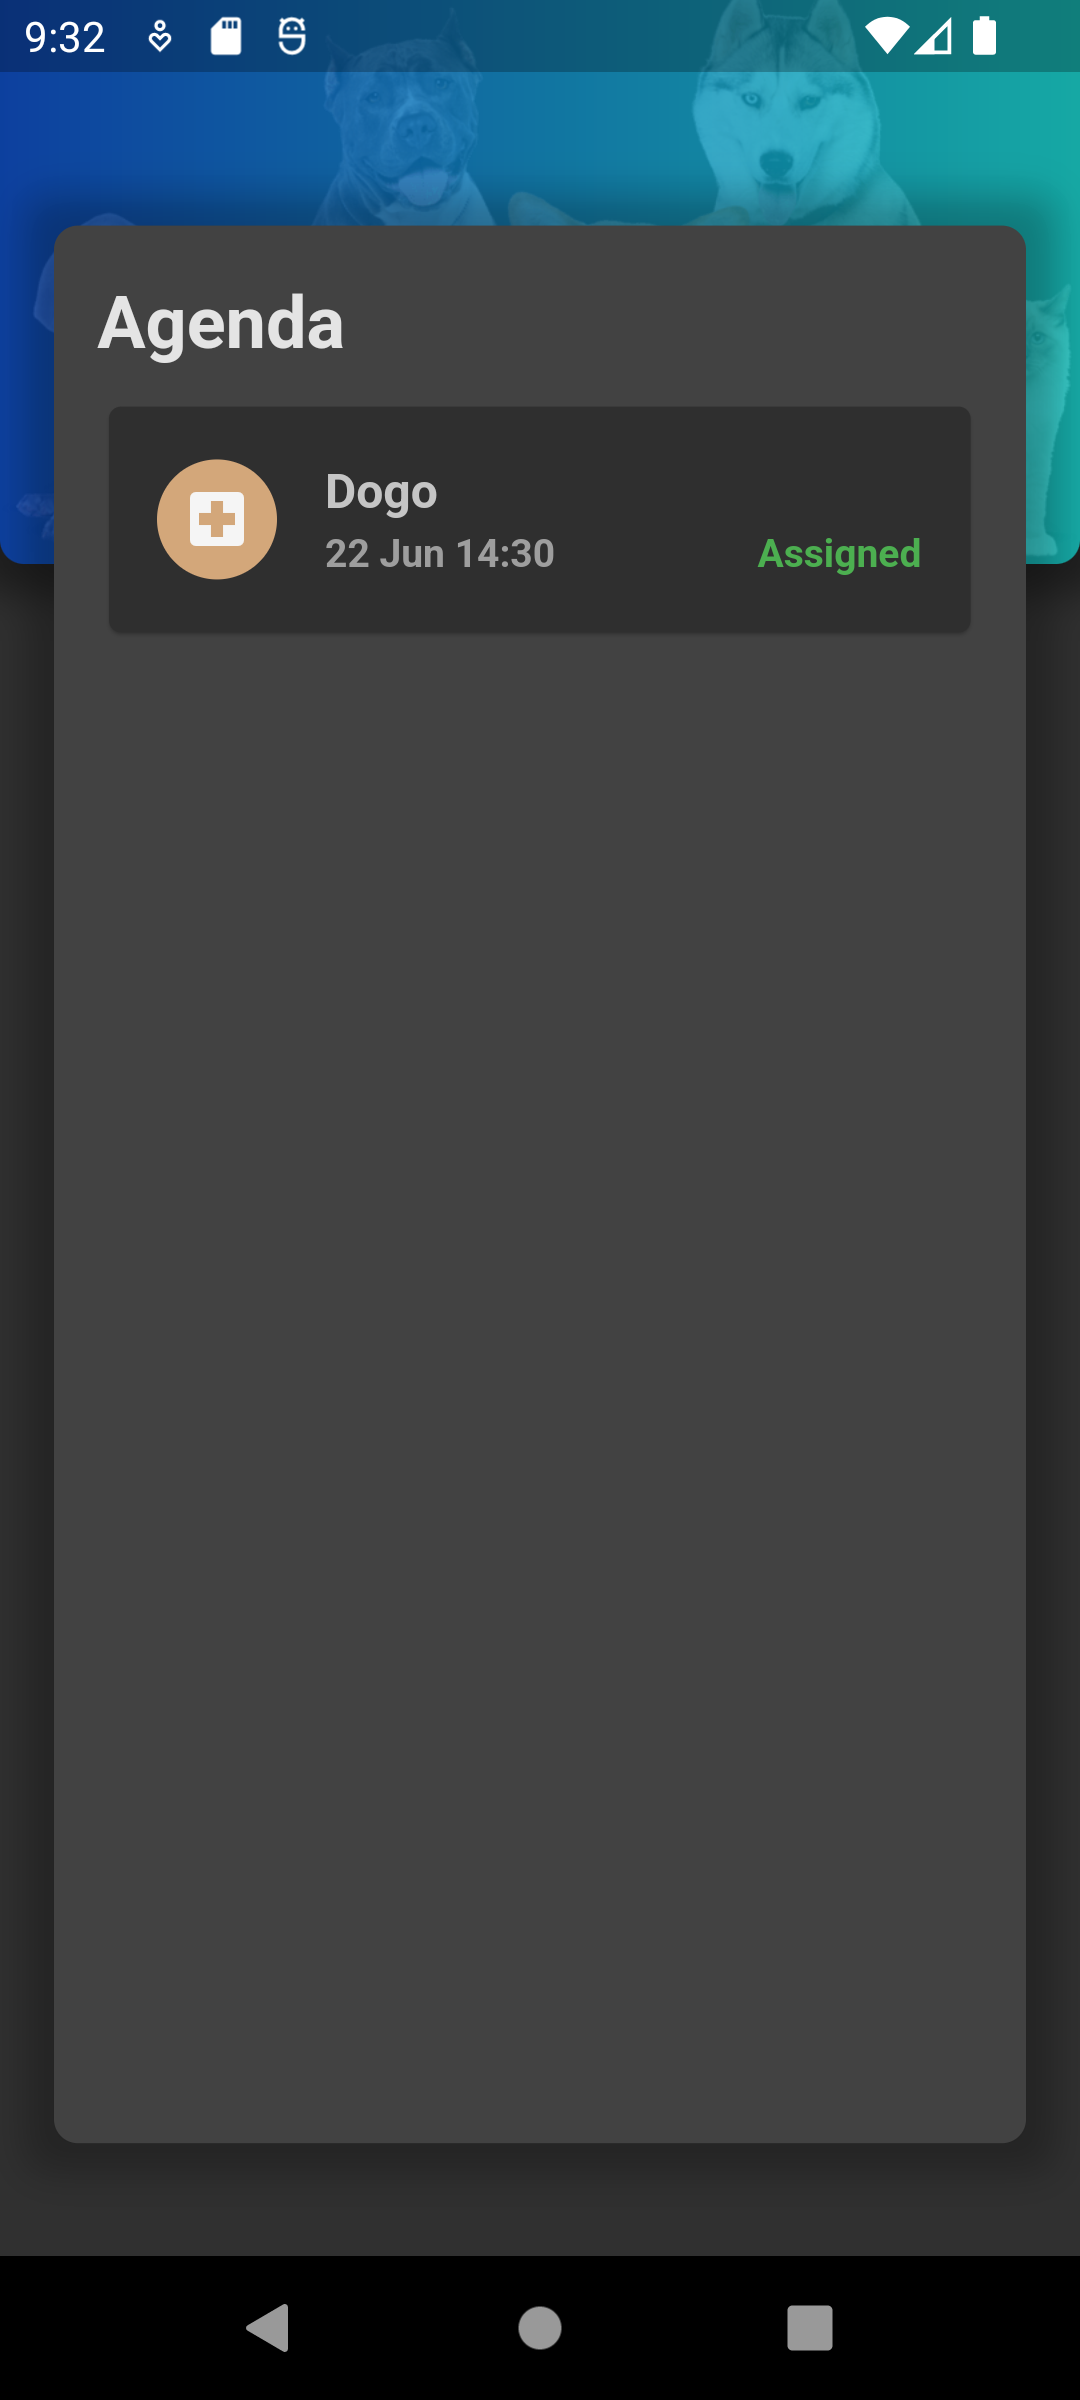
\includegraphics[width=0.31\textwidth]{images/screenshots/agenda.png}
    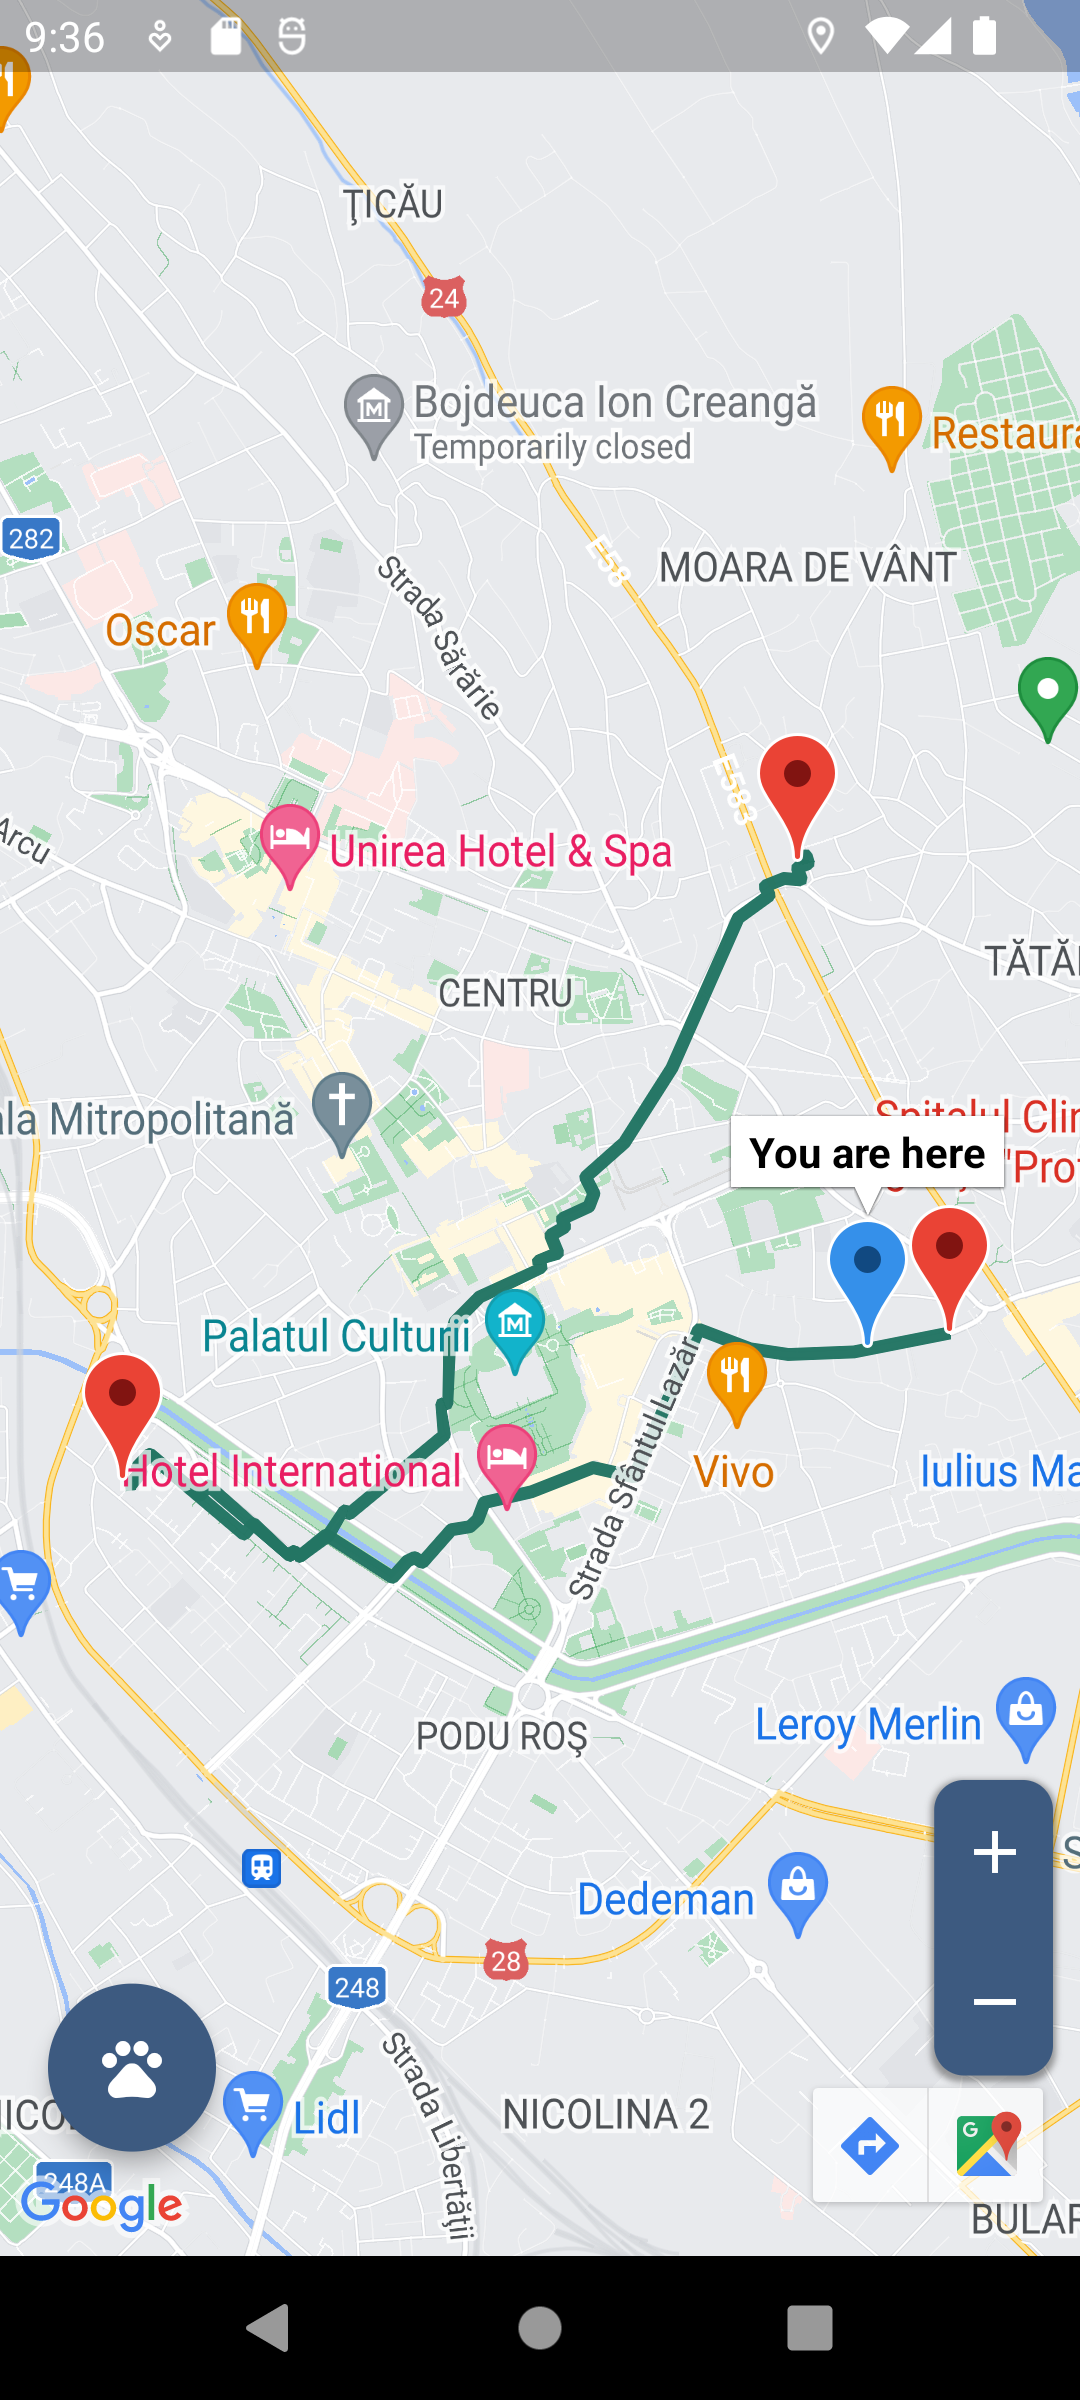
\includegraphics[width=0.31\textwidth]{images/screenshots/location_tracker.png}
    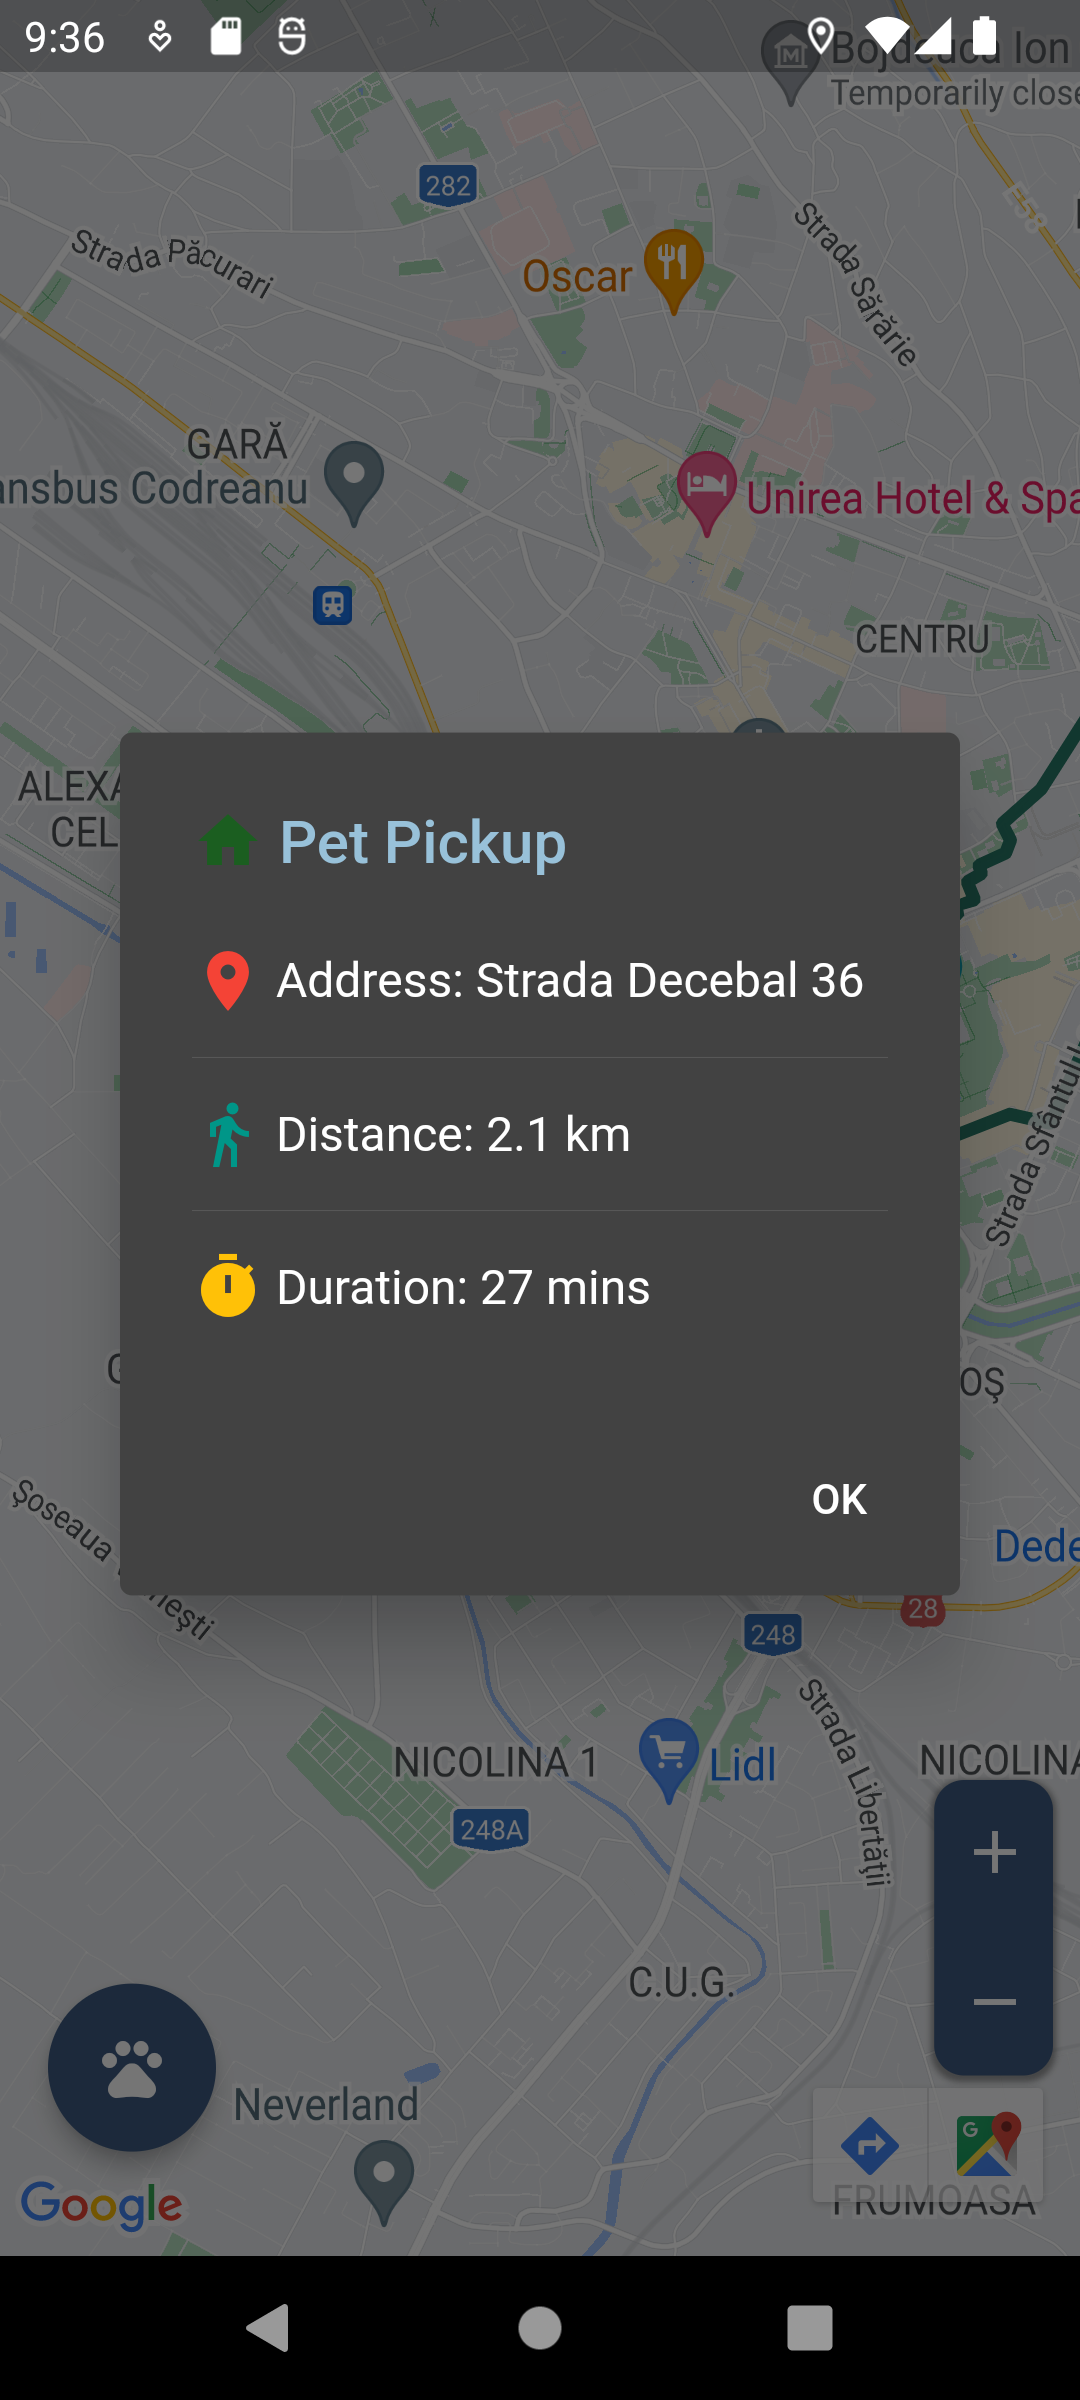
\includegraphics[width=0.31\textwidth]{images/screenshots/marker_info.png}
    \caption{Meniul „Your Agenda”}
    \label{fig:your_agenda}
\end{figure}


În figura \ref{fig:your_agenda} se poate observă meniul „Your Agenda” care conține lista de programări acceptate de utilizator. Dând click pe o programare va apărea harta care conține traseul generat al programării. În acest moment locația „Walker-ului” este urmărită constant, aceasta fiind reprezentată de bulina albastră. Dacă dăm click pe una din locațiile de pe harta, va apărea un meniu care ne prezintă informații despre distanța și timpul până la acea locația calculate folosind locația noastră actuală. Pentru a trece prin etapele unei programări în aplicația „Demo” ne vom folosi de butonul din partea stânga care ne va trece pe rând prin toate etapele până la finalizarea programării. Această funcționalitate nu va fi prezentă în aplicația finală deoarece „Walker-ul” va trebui să finalizeze programarea în momentul în care această este finalizată în realitate. 

De asemenea harta curentă poate fi vizualizată și de către „Owner-ul” animalului de companie, putând să urmărească în timp real desfășurarea programării.

